\documentclass[12pt,twoside]{book}
% \usepackage{cite}
% \usepackage[pdftex]{graphicx}
% \usepackage{array}
\usepackage{amsmath}
% \usepackage{bm}
% \usepackage{stmaryrd}
% \usepackage[tight,footnotesize]{subfigure}

\DeclareMathOperator*{\argmax}{arg\,max}
\DeclareMathOperator*{\argmin}{arg\,min}

\newcommand{\meutitulo}{Aprendizado ativo ... }
\newcommand{\meunome}{Davi Pereira dos Santos}
\newcommand{\meuorientador}{Prof. Dr. Andr� Carlos Ponce de Leon Ferreira de Carvalho}
\newcommand{\minhadata}{Dezembro/2014}
\newcommand{\minhabolsa}{Trabalho realizado com o apoio da CAPES.}
\newcommand{\meugrau}{Doutor}

%portugues
\usepackage[ruled,linesnumbered,vlined]{algorithm2e}
\usepackage{fancyhdr}

\usepackage{ textcomp }

%\renewcommand{\listalgorithmcfname}{Lista de Algoritmos}%
%\renewcommand{\algorithmcfname}{Algoritmo}%
\usepackage[english,brazil]{babel}
\usepackage{subfigure}
%%\usepackage{epigraph}
%%\usepackage{endnotes}
%\renewcommand{\notesname}{Coment�rios}
\usepackage{natbib}
\usepackage{latexsym}
\usepackage{setspace}
\usepackage{xspace}
% \usepackage[nohyperlinks]
%%% referencias com p�gina \vref
\usepackage[brazil]{varioref}
\usepackage{indentfirst}
%%% figuras um ao lado do outro
\usepackage{subfigure}
%%% definir t�tulos de se��o
\usepackage[sf,sl,outermarks]{titlesec}
\titleformat{\section}{\color{black}\normalfont\Large\bfseries}{\color{darkgray}\thesection}{1em}{}
\titleformat{\subsection}{\color{black}\normalfont\bfseries}{\color{darkgray}\thesubsection}{1em}{}

%%% boxes
\usepackage{fancybox}
\usepackage{fancyvrb}
\usepackage[usenames,dvipsnames]{color}
%\usepackage[pdftex]{graphicx}
\usepackage{graphicx}
\usepackage[pdftex]{geometry}
  \geometry{a4paper,left=3cm,right=2cm,top=2.0cm,bottom=2cm,twoside}

%%% cria links no arquivo .pdf
%%% comentar as linhas na vers�o para impressao
\usepackage[pdftex,pdfpagelabels,pagebackref,pageanchor=false]{hyperref}

% % Para imprimir PDFs com offset
% \begin{document}
% \begin{figure} %[H]
%     \centering
%     \includegraphics[bb=640 0 0 850]{/home/davi/12.pdf}
% %     \caption{\textit{Generative ensembles}}
% %     \label{gen}
% \end{figure}
% \end{document}


\usepackage{pdfpages}
\usepackage{multirow}
\hypersetup{
    pdftitle = {\meutitulo},
    pdfsubject = {},
    pdfkeywords = {},
    pdfauthor = {\meunome}
    }
\hypersetup{colorlinks=true,linkcolor=blue,citecolor=blue,hypertexnames=false}
% \usepackage[adobe-utopia]{mathdesign} %pacote texlive-fonts-extra no ubuntu
\usepackage{ae}
% \usepackage{bookman}
\usepackage[T1]{fontenc}
\usepackage{amsfonts}
\DeclareFixedFont{\numberfont}{T1}{phv}{bx}{n}{2cm}
\titleformat{\chapter}[display]
  {\normalfont\Large\sffamily
  }
  {%\titlerule[3pt]%
   \filright
   \rule[32pt]{.7\linewidth}{4pt}
   \hspace{-11pt}
   \shadowbox{
   \begin{minipage}{.18\linewidth}
     \begin{center}
       \textsc{\Large\chaptertitlename}\\
       \vspace{1ex}
       {\numberfont\color[gray]{0.5} \thechapter}\\
       \vspace{1ex}
     \end{center}
   \end{minipage}}
  }
  {0pt}
  {\filcenter
   \Huge
   }
  [\hfill\rule{.8\textwidth}{0.5pt}\\
     \vskip-1.8ex\hfill\rule{.7\textwidth}{3pt}]

\newcommand{\versal}[1]{{\noindent
    \setbox0\hbox{\largefont #1 }%
    \count0=\ht0                   % height of versal
    \count1=\baselineskip          % baselineskip
    \divide\count0 by \count1      % versal height/baselineskip
    \dimen1 = \count0\baselineskip % distance to drop versal
    \advance\count0 by 1\relax     % no of indented lines
    \dimen0=\wd0                   % width of versal
    \global\hangindent\dimen0      % set indentation distance
    \global\hangafter-\count0      % set no of indented lines
    \hskip-\dimen0\setbox0\hbox to\dimen0{\raise-\dimen1\box0\hss}%
    \dp0=0in\ht0=0in\box0}}

\definecolor{dark-green}{rgb}{0,0.5,0}
\newcommand{\X}{X\xspace}
\newcommand{\Y}{Y\xspace}
\newcommand{\xt}{\bm{x}_{(t)}\xspace}
\newcommand{\x}{\bm{x}\xspace}
\newcommand{\yt}{\bm{y}_{(t)}\xspace}
\newcommand{\y}{\bm{y}\xspace}
\newcommand{\pool}{reserva de exemplos\xspace}
\newcommand{\pools}{reservas de exemplos\xspace}
\newcommand{\U}{\mathcal{U}\xspace}
\newcommand{\Ut}{\U_{(t)}\xspace}
\newcommand{\Lt}{\mathcal{L}_{(t)}\xspace}
\newcommand{\tra}[2]{\underline{#1}\xspace\footnote{\textit{#2}\xspace}}
\newcommand{\blue}[1]{\textcolor{blue}{#1}\xspace}
\newcommand{\red}[1]{\textcolor{red}{#1}\xspace}
\newcommand{\green}[1]{\textcolor{dark-green}{#1}\xspace}
\newcommand{\esb}[1]{\blue{#1}\xspace}
\newcommand{\ano}[1]{\red{[$\star$ #1 $\star$]}\xspace}
\newcommand{\tar}[1]{\green{$\star$ #1}\xspace}
\newcommand{\versionspace}{espa�o de vers�es\xspace}

\newcommand{\ing}[2]{\emph{#1}\footnote{\textit{#2}}}
\newcommand{\novo}[1]{\emph{#1}}
\newcommand{\eer}{redu��o do erro esperado\xspace}
\newcommand{\Eer}{Redu��o do erro esperado\xspace}
\newcommand{\elms}{\textit{m�quinas extremas}\xspace}
\newcommand{\elm}{\textit{m�quina extrema}\xspace}
\newcommand{\svm}{m�quina de vetores de suporte\xspace}

\newcommand{\tarefa}[1] {\addcontentsline{toc}{section}{\tar{#1}}}







\newcommand{\emphFirst}[1] {\textbf{#1}}

\renewcommand{\reftextfacebefore}{}
\renewcommand{\reftextfaceafter}{}

\newcommand{\mx}{\hbox{\textbf{x}}\xspace}
\newcommand{\smx}{\hbox{{\scriptsize \textbf{x}}}\xspace}

\newcommand{\ranking}{\hbox{\textit{ranking}}\xspace}



% Backref com coloca��o de "Citado na p�gina..."
\renewcommand*{\backref}[1]{}
\renewcommand*{\backrefalt}[4]{
    \ifcase #1
        N�o citado no texto.
    \or
        Citado na p�gina~#2.
    \else
        Citado nas p�ginas #2.
    \fi
}

\renewcommand{\backreftwosep}{ e~}
\renewcommand{\backreflastsep}{, e~}


\hyphenation{su-per-vi-sio-na-dos}
\hyphenation{su-per-vi-sio-na-do}


\newcommand{\gnuplot}{\textbf{GnuPlot$^{TM}$}\xspace}
\newcommand{\tfidf}{\textit{tfidf}\xspace}
\newcommand{\tflinear}{\textit{tflinear}\xspace}




\newcommand{\smooth}{\emph{smooth}\xspace}

\newcommand{\stempl}{\textbf{stem.pl}\xspace}
\newcommand{\reportpl}{\textbf{report.pl}\xspace}
\newcommand{\predictpl}{\textbf{predict.pl}\xspace}
\newcommand{\stembase}{\textbf{stembase}\xspace}
\newcommand{\textbase}{\textbf{textbase}\xspace}
\newcommand{\stoplist}{\textbf{stoplist}\xspace}


\newcommand{\sone}{\texttt{\%one\%}\xspace}
\newcommand{\stwo}{\texttt{\%two\%}\xspace}
\newcommand{\sthree}{\texttt{\%three\%}\xspace}
\newcommand{\sglobal}{\texttt{\%global\%}\xspace}
\newcommand{\stm}{\textit{stemming}\xspace}
\newcommand{\stemming}{\textit{stemming}\xspace}
\newcommand{\gram}{\textit{gram}\xspace}
\newcommand{\grams}{\textit{grams}\xspace}

\newcommand{\stems}{\textit{stems}\xspace}
\newcommand{\stem}{\textit{stem}\xspace}
\newcommand{\pretext}{\textsc{PreTexT}\xspace}
\newcommand{\script}{\textit{script}\xspace}
\newcommand{\scripts}{\textit{scripts}\xspace}
\newcommand{\stoplists}{\textit{stoplists}\xspace}
\newcommand{\stopfile}{\textit{stopfile}\xspace}
\newcommand{\stopfiles}{\textit{stopfiles}\xspace}
\newcommand{\stopword}{\textit{stopword}\xspace}
\newcommand{\stopwords}{\textit{stopwords}\xspace}


% experimentos
\newcommand{\news}{{\sc news}\xspace}
\newcommand{\course}{{\sc course}\xspace}
\newcommand{\lnai}{{\sc lnai}\xspace}
\newcommand{\ccourse}{{\tt course}\xspace}
\newcommand{\cncourse}{{\tt non-course}\xspace}
\newcommand{\sci}{{\tt sci}\xspace}
\newcommand{\talk}{{\tt talk}\xspace}
\newcommand{\texto}{\textsc{texto}\xspace}
\newcommand{\links}{\textsc{links}\xspace}

\newcommand{\cbr}{\textsc{cbr}\xspace}
\newcommand{\ilp}{\textsc{ilp}\xspace}





\newcommand{\kmeanski}
  {$k$-{\it means}$_{ki}$\xspace}

\newcommand{\kmeans}
  {$k$-me\-ans\xspace}


\newcommand{\clustering}
  {\textit{clustering}\xspace}



\newcommand{\kparticoes}
  {$k$-parti��es\xspace}

\newcommand{\coboosting}
  {\textsc{CO-BOOSTING}\xspace}

\newcommand{\boosting}
  {{\em Boosting}\xspace}


\newcommand{\bagging}
  {{\em Bagging}\xspace}

\newcommand{\naivebayes}
  {\emph{Naive Bayes}\xspace}

\newcommand{\bayes}
  {{\em Bayes}\xspace}

\newcommand{\framework}
  {\textsc{framework}\xspace}


% bullet
\newcommand{\bb}
  {\ensuremath{\bullet}}

% neck
\newcommand{\neck}
  {{\texttt{\bf\ :-\ }}}

% circ
\newcommand{\cc}
  {\ensuremath{\circ}}

% diamond
\newcommand{\dd}
  {\ensuremath{\diamond}}

% MLC++
\newcommand{\mlc}
  {\ensuremath{\mathcal{MLC\hspace{-.05em}\raisebox{.4ex}{\tiny\bf ++}}}\xspace}

% MySQL
\newcommand{\mysql}
%  {{\sc \smaller MySQL}\xspace}
  {\ensuremath{\mathcal{M}{\sf y}\mathcal{SQL}}\xspace}

% C++
\newcommand{\cplusplus}
  {\ensuremath{\mathcal{C\hspace{-.05em}\raisebox{.4ex}{\tiny\bf ++}}}\xspace}

% C++
\newcommand{\cpp}
  {\cplusplus}

% CI
\newcommand{\ci}
  {\ensuremath{\mathcal{CI}}\xspace}
%  {{\sc ci}\xspace}

% ID3
\newcommand{\idtree}
%  {{\sc id\relsize{-2}3}\xspace}
  {\ensuremath{\mathcal{ID}3}\xspace}

% GID3*
\newcommand{\gidtree}
  {{\sc gid\relsize{-2}3*}\xspace}

% Skicat
\newcommand{\skicat}
  {{\sc \smaller Skicat}\xspace}

% PBM
%\newcommand{\pbm}
 % {{\sc \smaller pbm}\xspace}

%PBM
\newcommand{\pbm}
   {\ensuremath{\mathcal{PBM}}\xspace}

% C4.5
\newcommand{\cfourfive}
%  {{\sc c\relsize{-2}4.5}\xspace}
  {\ensuremath{\mathcal{C}4.5}\xspace}

% C4.5rules
\newcommand{\cfourfiverules}
%  {{\sc c{\relsize{-2}4.5}rules}\xspace}
  {\ensuremath{\mathcal{C}4.5{\sf rules}}\xspace}

% C4.5-rules
\newcommand{\cfourfiver}
  {{\sc c{\relsize{-2}4.5}rules}\xspace}
%  {\ensuremath{\mathcal{C}4.5{\sf rules}}\xspace}

% C4.5r
\newcommand{\cfourfiverr}
  {{\sc c{\relsize{-2}4.5}r}\xspace}
%  {\ensuremath{\mathcal{C}4.5{\sf r}}\xspace}

% C5.0
\newcommand{\cfive}
%  {{\sc c\relsize{-2}5.0}\xspace}
  {\ensuremath{\mathcal{C}5.0}\xspace}

% See5
%\newcommand{\seefive}
%  {{\sc see\relsize{-2}5}\xspace}
%  {\ensuremath{\mathcal{S}}{\sf ee5}\xspace}

% See5
\newcommand{\seefive}
  {\ensuremath{\mathcal{S}}{\sf ee5}\xspace}


% CN2
\newcommand{\cntwo}
 % {{\sc cn\relsize{-2}2}\xspace}
  {\ensuremath{\mathcal{CN}2}\xspace}

% OC1
\newcommand{\ocone}
%  {{\sc oc\relsize{-2}1}\xspace}
  {\ensuremath{\mathcal{OC}1}\xspace}

% T2
%\newcommand{\ttwo}
 % {{\sc t\relsize{-2}2}\xspace}

% MC4
%\newcommand{\mcfour}
 % {{\sc mc\relsize{-2}4}\xspace}

%MC4
\newcommand{\mcfour}
  {\ensuremath{\mathcal{MC}4}\xspace}

%T2
\newcommand{\ttwo}
  {\ensuremath{\mathcal{T}2}\xspace}

% RIPPER
\newcommand{\ripper}
%  {{\sc ripper}\xspace}
  {\ensuremath{\mathcal{R}}{\sc \em ipper}\xspace}

% Progol
\newcommand{\progol}
  {{\sc progol}\xspace}

% Naive Bayes
\newcommand{\nb}
  {{\sc nb}\xspace}

% Instance Based
\newcommand{\ib}
  {{\sc ib}\xspace}

% Labic
\newcommand{\labic}
  {{\sc labic}\xspace}

% Ruler
\newcommand{\ruler}
  {{\sc ruler}\xspace}

% Xruler
\newcommand{\xruler}
  {{\sc xruler}\xspace}

% Discover
\newcommand{\discover}
  {\textsc{Discover}}

% perl
\newcommand{\perl}
  {{\sc perl}\xspace}


% O-BTree
\newcommand{\obtree}
  {{\sc o-btree}\xspace}

% Focas
\newcommand{\focas}
  {{\sc focas}\xspace}

% Focus
\newcommand{\focus}
  {{\sc focus}\xspace}

% Relief
\newcommand{\relief}
  {{\sc relief}\xspace}


% Foil
\newcommand{\foil}
  {{\sc foil}\xspace}

% CART
\newcommand{\cart}
  {{\sc cart}\xspace}

% BibTeX
\def\BibTeX{{\rm B\kern-.05em{\sc i\kern-.025em b}\kern-.08em
    T\kern-.1667em\lower.7ex\hbox{E}\kern-.125emX}\xspace}
% BibTeX
\def\bibtex{\BibTeX}

% BibView
\def\BibView{{\rm B\kern-.05em{\sc i\kern-.025em b}\kern-.08em
    V\kern-.1667em\hbox{\sc iew}}\xspace}
\def\bibview{\BibView}

% Nro
\newcommand{\nro}
  {\scriptsize $^{\b{o}}$\normalsize\xspace}

% Nra
\newcommand{\nra}
  {\scriptsize $^{\b{a}}$\normalsize\xspace}

% e.g.
\newcommand{\eg}
  {{\em e.g.}\/\xspace}

% i.e.
\newcommand{\ie}
  {{\em i.e.}\/\xspace}

% trademark
\newcommand{\TM}
  {\footnotesize\ensuremath{^{\rm TM}}\normalsize\xspace}
\newcommand{\tm}
  {\TM}

%\newcommand{\IF}
%  {{\bf IF}\xspace}
\newcommand{\THEN}
  {{\bf THEN}\xspace}
% and
\newcommand{\AND}
  {{\bf AND}\xspace}
% proc
\newcommand{\PROC}
  {{\bf procedure}\xspace}
% return
\newcommand{\RETURN}
  {{\bf return}\xspace}
% in
\newcommand{\IN}
  {{\bf in}\xspace}
% in
\newcommand{\REM}[1]
  {\hspace*{1cm}{\em // #1}\xspace}


% Palavras em ingles
%\newcommand{\engl}[1]
%  {{\em#1}}
%  {\selectlanguage{english}{\em#1}\selectlanguage{brazil}}

% URL
%\newcommand{\url}[1]
%  {{\tt #1}\xspace}

\newcommand{\ip}[2]
  {(#1, #2)}

\newcommand{\seq}[3][X,1,n]
  {\lbrace #1_{#2},\ldots,\,#1_{#3} \rbrace}

\newcommand{\cartesiano}[3][X,1,n]
  {#1_{#2} \times \ldots \times #1_{#3}}

% entrada de indice simples
\newcommand{\idxa}[1]
  {#1\index{#1}}

% entrada de indice dupla
\newcommand{\idxb}[2]
  {#1 #2\index{#1!#2}}

% entrada de indice tripla
\newcommand{\idxc}[3]
  {#1 #2 #3\index{#1!#2!#3}}

% PCTeX
% figura x-size y-size filename extension label caption
%          1      2       3        4         5      6

% PCTeX
% figura x-size y-size filename extension label caption
%          1      2       3        4         5      6
\newcommand{\figura}[6]
{\begin{figure}[hbt]
   \vspace*{0.5cm}
   \setlength{\unitlength}{1.0cm}
   \centering
   \begin{picture}(#1, #2)(0, 0)
     \special{#4:./#3.#4 x=#1cm y=#2cm}
   \end{picture}
   \caption{#6}
   \label{#5}
 \end{figure}
}

%%% inclus�o de figuras
% \figurajpg{escala}{nome.extensao}{label}{caption}
\newcommand{\figurajpg}[5]
{\begin{figure}[!h]
   \setlength{\unitlength}{1.0cm}
   \centering
     \includegraphics[scale=#1]{#2}
   \caption{#3}
   \label{#4}
 \end{figure}
}

\newcommand{\figurajpgg}[5]
{\begin{figure}[!hbt]
   \setlength{\unitlength}{1.0cm}
   \centering
     \includegraphics[scale=#1]{#2}
   \caption[#5]{#4}
   \label{#3}
 \end{figure}
}

%\newcommand{\figurac}[7]
%{\begin{figure}[hbt]
 %  \vspace*{0.5cm}
 %  \setlength{\unitlength}{1.0cm}
 %  \centering
 %  \begin{picture}(#1, #2)(0, 0)
 %    \special{#4:./#3.#4 x=#1cm y=#2cm}
 %  \end{picture}
 %  \caption[#7]{#6}
 %  \label{#5}
 %\end{figure}
%}


\newcommand{\figuraa}[6]
{\begin{figure}
%   \vspace*{1cm}
   \setlength{\unitlength}{1.0cm}
   \centering
   \begin{picture}(#1, #2)(0, 0)
     \special{#4:./#3.#4 x=#1cm y=#2cm}
   \end{picture}
   \caption{#6}
   \label{#5}
 \end{figure}
}

\newcommand{\figurah}[6]
{\begin{figure}[htb]
%   \vspace*{0.2cm}
   \setlength{\unitlength}{1.0cm}
   \centering
   \begin{picture}(#1, #2)(0, 0)
     \special{#4:./#3.#4 x=#1cm y=#2cm}
   \end{picture}
   \caption{#6}
   \label{#5}
 \end{figure}
}

\newcommand{\figuraH}[6]
{\begin{figure}[H]
%   \vspace*{0.2cm}
   \setlength{\unitlength}{1.0cm}
   \centering
   \begin{picture}(#1, #2)(0, 0)
     \special{#4:./#3.#4 x=#1cm y=#2cm}
   \end{picture}
   \caption{#6}
   \label{#5}
 \end{figure}
}

\newcommand{\figurat}[6]
{\begin{figure}[tbh]
%   \vspace*{1cm}
   \setlength{\unitlength}{1.0cm}
   \centering
   \begin{picture}(#1, #2)(0, 0)
     \special{#4:./#3.#4 x=#1cm y=#2cm}
   \end{picture}
   \caption{#6}
   \label{#5}
 \end{figure}
}

\newcommand{\figurab}[6]
{\begin{figure}[bth]
%   \vspace*{0.2cm}
   \setlength{\unitlength}{1.0cm}
   \centering
   \begin{picture}(#1, #2)(0, 0)
     \special{#4:./#3.#4 x=#1cm y=#2cm}
   \end{picture}
   \caption{#6}
   \label{#5}
 \end{figure}
}

\newcommand{\figurac}[7]
{\begin{figure}[hbt]
   \vspace*{0.5cm}
   \setlength{\unitlength}{1.0cm}
   \centering
   \begin{picture}(#1, #2)(0, 0)
     \special{#4:./#3.#4 x=#1cm y=#2cm}
   \end{picture}
   \caption[#7]{#6}
   \label{#5}
 \end{figure}
}

\newcommand{\myquotation}[2]{%
  %\vspace{0.5ex}%
  {\singlespacing
    \footnotesize%
    \begin{flushright}%
      \begin{minipage}{.5\textwidth}%
        {\sf \noindent \textcolor{RawSienna}{#1}}\\
      \end{minipage}\\
      \textit{\noindent \textcolor{RawSienna}{#2}}%
    \end{flushright}}%
  %\vspace{0.5ex}
  }

%\myquotation{``Smoking kills. If you're killed, you've lost a very important part of your life.''}{Brooke Shields.}



% < x >
\newcommand{\braces}[1]
  {$<$#1$>$\xspace}

% Palavras em ingles

% | - ou
\newcommand{\ou}
   {$|$\xspace}

% e-mail
%\newcommand{\email}
%   {\begingroup \urlstyle{tt}\Url}


\newcommand{\inducer}[1]
  {\ensuremath{\mathcal{I\hspace{-.05em}}^{#1}}\xspace}

\newcommand{\dataset}[1]
  {\ensuremath{\mathcal{D\hspace{-.05em}}^{#1}}\xspace}

\newcommand{\classifier}[1]
  {\ensuremath{\mathcal{C\hspace{-.05em}}^{#1}}\xspace}



% \usepackage{parallel} % para as equa��es de medidas multilabel

%%%%%%%%%%%%%%%% FORMATACAO DE PALAVRAS %%%%%%%%%%%%%%%%%%%%%

\newcommand{\nf }[1] % nome de ferramenta
    {\textsc{#1}}
\newcommand{\pe }[1] % termo em ingl�s
    {\textit{#1}}

%%%%%%%%%%%%%%%%%%%%%%%%%%%%%%%%%%%%%%%%%%%%%%%%%%%%%%%%%
\usepackage{ctable}
\newcommand{\RAKEL}{{\emph {RAKEL}}\/\xspace}
\newcommand{\win}{{+}\/\xspace}
\newcommand{\lose}{{-}\/\xspace}
\usepackage{amsmath}

% \usepackage[usenames,dvipsnames]{xcolor}
\definecolor{cinzaclaro}{rgb}{0.84,0.84,0.84}
\newcommand{\e}{\colorbox{cinzaclaro}}


%inkscape svg auto refresh - adicionar -shell-escape na chamada de pdflatex
% \newcommand{\executeiffilenewer}[3]{
% \ifnum\pdfstrcmp{\pdffilemoddate{#1}}
% {\pdffilemoddate{#2}}>0
% {\immediate\write18{#3}}\fi
% }
% \newcommand{\includesvg}[1]{
% \executeiffilenewer{#1.svg}{#1.pdf}
% {inkscape -z -D --file=#1.svg
% --export-pdf=#1.pdf --export-latex}
% \input{#1.pdf_tex}
% }

% \pgfdeclareplotmark{v}{%
%   \pgfpathmoveto{\pgfpoint{-\pgfplotmarksize}{\pgfplotmarksize}}
%   \pgfpathlineto{\pgfpoint{0pt}{0pt}}
%   \pgfpathlineto{\pgfpoint{\pgfplotmarksize}{\pgfplotmarksize}}
%   \pgfusepathqstroke
% }
% \pgfdeclareplotmark{^}{%
%   \pgfpathmoveto{\pgfpoint{-\pgfplotmarksize}{-\pgfplotmarksize}}
%   \pgfpathlineto{\pgfpoint{0pt}{0pt}}
%   \pgfpathlineto{\pgfpoint{\pgfplotmarksize}{-\pgfplotmarksize}}
%   \pgfusepathqstroke
% }

\usepackage{amssymb}
\usepackage{pgfplots,bm}
\usetikzlibrary{plotmarks}
\usetikzlibrary{scopes,shapes,shadows,calc,arrows,shapes.symbols,automata,decorations.pathmorphing,backgrounds,fit,positioning}
\usetikzlibrary{external}
\tikzexternalize

% styles for flowcharts
\tikzstyle{d} = [diamond, draw, text width=4.5em, text badly centered, node distance=3cm, inner sep=0pt]
\tikzstyle{block} = [rectangle, draw, text width=3em, text centered, rounded corners, minimum height=4em]
\tikzstyle{s} = [-triangle 60,thick]
\tikzstyle{b} = [rectangle, thick, draw, aspect=3, shape border rotate=90, minimum height=1, rounded corners, minimum width=1, outer sep=-0.5\pgflinewidth, color=black, top color=black!10, bottom color=black!10, middle color=white]
\tikzstyle{ensemble} = [text height=1, rectangle, thick, draw, aspect=3, shape border rotate=90, minimum height=100, rounded corners, minimum width=100, outer sep=-0.5\pgflinewidth, color=black, top color=black!10, bottom color=black!10, middle color=white]
\tikzstyle{aprendizst} = [text height=1, rectangle, thick, draw, aspect=3, shape border rotate=90, minimum height=10, rounded corners, minimum width=10, outer sep=-0.5\pgflinewidth, color=black, top color=black!15, bottom color=white]
\tikzstyle{bdtr} = [cylinder, thick, draw, aspect=1, shape border rotate=90, minimum height=45, minimum width=40, outer sep=-0.5\pgflinewidth, color=black, left color=blue!40, right color=blue!40, middle  color=white]
\tikzstyle{bdts} = [cylinder, thick, draw, aspect=1, shape border rotate=90, minimum height=45, minimum width=40, outer sep=-0.5\pgflinewidth, color=black, left color=orange!40, right color=orange!40, middle  color=white]

\def\ctr [#1,#2]#3{
  \node (#1) [bdtr, #3] #2 {$\mathcal{L}$} ;
}

\def\cts [#1,#2]#3{
  \node (#1) [bdts, #3] #2 {$\mathcal{U}$} ;
}

\tikzstyle{nuvem}=[cloud, thick, draw, cloud puffs=12, aspect=5, alias=cyl, shape border rotate=90, minimum height=50, minimum width=60, outer sep=-0.5\pgflinewidth, color=black, top color=orange!40, bottom color=orange!40, middle  color=white]
\def\fluxo [#1,#2]#3{
  \node (#1) [nuvem, #3] #2 {fluxo de dados};
}
\pgfdeclarelayer{ss3} \pgfdeclarelayer{ss2} \pgfdeclarelayer{ss1}
\pgfdeclarelayer{pi3} \pgfdeclarelayer{pi2} \pgfdeclarelayer{pi1}
\pgfdeclarelayer{main}
\pgfsetlayers{ss3,ss2,ss1,main,pi1,pi2,pi3}

\tikzset{seta/.style={solid, ultra thick, black}}
\tikzset{setatr/.style={solid, ultra thick, blue}}
\tikzset{setats/.style={dashed, ultra thick, orange}}

\newcommand*\C[1]{
  \begin{tikzpicture}
      \node[draw,circle,inner sep=1pt] {#1};
  \end{tikzpicture}
}
\newcommand*\Q[1]{
  \begin{tikzpicture}
      \node[draw,rectangle,inner sep=2pt] {#1};
  \end{tikzpicture}
}
\newcommand*\T[1]{
  \begin{tikzpicture}
%       \node[draw,circle,inner sep=2pt] {#1};
      \node[draw,circle,inner sep=1.5pt] {#1};
      \node[draw,circle,inner sep=2.5pt] {#1};
       \node[black, thick, inner sep=2pt] {#1};
  \end{tikzpicture}
}

\def\estrutura [#1,#2]#3{
	\node (#1) [#3] #2{
	\begin{tikzpicture}[node distance=90, auto, >=stealth, scale=0.15, transform shape]
	  \node (ei#1) [d, thick] {};
	  \node (ei2#1) [below right of=ei#1, block, thick] {};
	  \node (ei3#1) [below left of=ei#1, block, thick] {};
	  \draw[->, seta] (ei#1.south east)  -- node[left=1] {} (ei2#1.west);
	  \draw[->, seta] (ei#1.south west)  -- node[left=1] {} (ei3#1.east);
	  \begin{pgfonlayer}{ss1}
	    \node (ax#1)  [draw, circle, fit=(ei#1) (ei2#1) (ei3#1), inner sep=1, scale=1, thick, top color=white, bottom color=white, middle color=black!10] {};
	  \end{pgfonlayer}
	\end{tikzpicture}
	};
}

\def\fronteira [#1,#2]#3{
	\node (#1) [#3] #2{
	\begin{tikzpicture}[node distance=0, auto, >=stealth, scale=0.2, transform shape]
		      \pgfplotsset{width=7cm}
		      \pgfplotsset{samples at={30.1,30.2,...,65}}
					\begin{axis} [name=ei#1,xmin=30, xmax=70, ymin=1.5, ymax=1.85, axis y line=left, axis x line=bottom] %,xlabel=peso (kg),   ylabel=altura (m)]
					\addplot[only marks,mark=*,mark options={blue, ultra thick, scale=5}] plot coordinates {				  (65,1.8) (54,1.75) (63,1.6) (72,1.65) (50,1.8) (62,1.68)  (77,1.71)				      };
					\addplot[only marks,mark=o,mark options={ultra thick,red,scale=5}] plot coordinates {				  (35,1.7) (39,1.60) (50,1.60) (58,1.54) (46,1.67) (43,1.55)				      };
					\addplot [only marks, mark=*, mark options={teal, ultra thick,scale=2}] {2.36 -x/(131/1.7)};
					\end{axis}
		\begin{pgfonlayer}{ss1}
			  \node (ax#1)  [draw, circle, fit=(ei#1), inner sep=1, scale=1, thick, top color=white, bottom color=white, middle color=black!10] {};
		\end{pgfonlayer}
	\end{tikzpicture}
	};
}


\def\algtrein[#1,#2,#3]#4{
		\node (#1) [b, label=-90:
% \begin{tabular}{c}
  alg. trein.#3
% \end{tabular}
, #4] #2{
			$a_{#3}( \theta_#3^{(t-1)}, \langle \bm{x},y \rangle )$
		};
}

\def\classificador[#1,#2,#3]#4{
		\node (#1) [b, label=-90:$h_#3^{(t)}$, #4] #2{
				$\argmax_y\{ P_{\theta_#3} (y|\bm{x})\}$
		};
}

\def\classificadorprob[#1,#2,#3]#4{
		\node (#1) [b, label=-90:${ }_#3$, #4] #2{
				$\max_{y \in Y}\{P_{\theta_#3} (y|\bm{x})\}$
		};
}

\def\aprendiz [#1,#2,#3]#4{
	\node (#1) [label distance=-2, #4,label=-90:aprendiz passivo #3] #2{
	\begin{tikzpicture}[node distance=0, auto, scale=1, transform shape,remember picture, text centered]
				\algtrein [a#1,  , #3] {}
				\tikzset{label distance=-8, node distance=85}
				\estrutura [f#1, ] {label=-90:$\theta_{#3}^{(t)}$, right of=a#1}
				\tikzset{label distance=-2, node distance=100}
				\classificador [c#1, , #3] {right of=f#1}
				\draw[->,setatr] (a#1) -- node (1,1)[] {} (f#1);
 			   \draw[<->, setats] (f#1)  -- node[left=1] {} (c#1);
%  			   \draw[->, ultra thick] (c#1)  to [out=110,in=60] node[] {} (f#1);
			\begin{pgfonlayer}{ss2}
			\node (aa#1) [aprendizst, fit = (a#1) (f#1)(c#1), inner sep=10] {} ;
			\end{pgfonlayer}
%  		   \draw[->, ultra thick] (aa#1.west)  -- node[] {} (a#1);
	\end{tikzpicture}
	};
}

\def\homem [#1,#2]#3{
  \node (#1) [#3] #2{
  \begin{tikzpicture}[node distance=0, auto, >=stealth, scale=0.77, transform shape]
    \node (cabeca) [draw, circle, inner sep=3, ultra thick] {. .};
    \node (umbigo) [circle,below=1.2 of cabeca] {};
    \node (tronco) [circle,below=0.3 of cabeca] {};
    \draw[-, seta] (cabeca.south)  to [out=-90,in=90] node[] {} (umbigo);
    \node (pesq) [circle,below left=0.5 of umbigo] {};
    \node (pdir) [circle,below right=0.5 of umbigo] {};
    \draw[-, seta] (pesq)  to  node[] {} (umbigo.north);
    \draw[-, seta] (pdir)  to  node[] {} (umbigo.north);
    \node (mesq) [circle,below left=0.5 of cabeca] {};
    \node (mdir) [circle,below right=0.5 of cabeca] {};
    \draw[-, seta] (mesq)  to  node[] {} (tronco.north);
    \draw[-, seta] (mdir)  to  node[] {} (tronco.north);
    \begin{pgfonlayer}{ss2}
      \node (fit#1) [b, draw, fit = (cabeca) (pesq) (pdir)] {};
    \end{pgfonlayer}
  \end{tikzpicture}
  };
}

\def\modeloprob [#1,#2,#3]#4{
	\node (#1) [label distance=-2, #4,label=-90:aprendiz #3] #2{
	\begin{tikzpicture}[node distance=0, auto, scale=1, transform shape,remember picture, text centered]
				\algtrein [a#1,  , #3] {}
				\tikzset{label distance=-8, node distance=85}
				\estrutura [f#1, ] {label=-90:$\theta_#3^{(t)}$, right of=a#1}
				\tikzset{label distance=-2, node distance=100}
				\classificadorprob [c#1, , #3] {right of=f#1}
				\draw[->,setatr] (a#1) -- node (1,1)[] {} (f#1);
 			   \draw[<->, setats] (f#1)  -- node[left=1] {} (c#1);
%  			   \draw[->, ultra thick] (c#1)  to [out=110,in=60] node[] {} (f#1);
			\begin{pgfonlayer}{ss2}
					\node (aa#1) [aprendizst, fit = (a#1) (f#1)(c#1), inner sep=12] {} ;
			\end{pgfonlayer}
%  		   \draw[->, ultra thick] (aa#1.west)  -- node[] {} (a#1);
	\end{tikzpicture}
	};
}

% version space
\def\modelovs [#1,#2,#3]#4{
	\node (#1) [label distance=-2, #4,label=-90:aprendiz #3] #2{
	\begin{tikzpicture}[node distance=0, auto, scale=1, transform shape,remember picture, text centered]
				\algtrein [a#1,  , #3] {}
				\tikzset{label distance=-8, node distance=85}
				\estrutura [f#1, ] {label=-90:$\theta_#3^{(t)}$, right of=a#1}
				\tikzset{label distance=-2, node distance=100}
				\node (c#1) [b, right of=f#1, label=-90:$\textit{version space}$] {
  \begin{tabular}{ll}
    $\bf{x}$ que melhor define \\
    hipóteses válidas
  \end{tabular}
};
				\draw[->,setatr] (a#1) -- node (1,1)[] {} (f#1);
%  			   \draw[->, ultra thick] (c#1)  to [out=110,in=60] node[] {} (f#1);
			\begin{pgfonlayer}{ss2}
					\node (aa#1) [aprendizst, fit = (a#1) (f#1)(c#1), inner sep=12] {} ;
			\end{pgfonlayer}
%  		   \draw[->, ultra thick] (aa#1.west)  -- node[] {} (a#1);
	\end{tikzpicture}
	};
}

% \usepackage{glosstex}
\usepackage[printonlyused,withpage]{acronym}

\begin{document}
\input tarefas
\pagestyle{empty}
\pagenumbering{roman}
\newcommand{\titulo}{\meutitulo}
\newcommand{\autor}{\meunome}
\newcommand{\orientador}{\meuorientador}
\newcommand{\nota}{Tese apresentada ao Instituto de Ci�ncias Matem�ticas e de Computa��o - ICMC-USP, para o Exame de Qualifica��o, como parte dos requisitos necess�rios � obten��o do t�tulo de \meugrau\xspace em Ci�ncias de Computa��o e Matem�tica Computacional.}
%\newcommand{\nota}{Monografia apresentada � disciplina de Metodologia de Pesquisa Cient�fica em Intelig�ncia Artificial, no Instituto de Ci�ncias Matem�ticas e de Computa��o - ICMC-USP, como parte dos requisitos necess�rios � obten��o dos cr�ditos relacionados � disciplina.}

\newcommand{\data}{\minhadata}
\newcommand{\comentario}{\minhabolsa}
\tikzexternaldisable
\begin{titlepage}
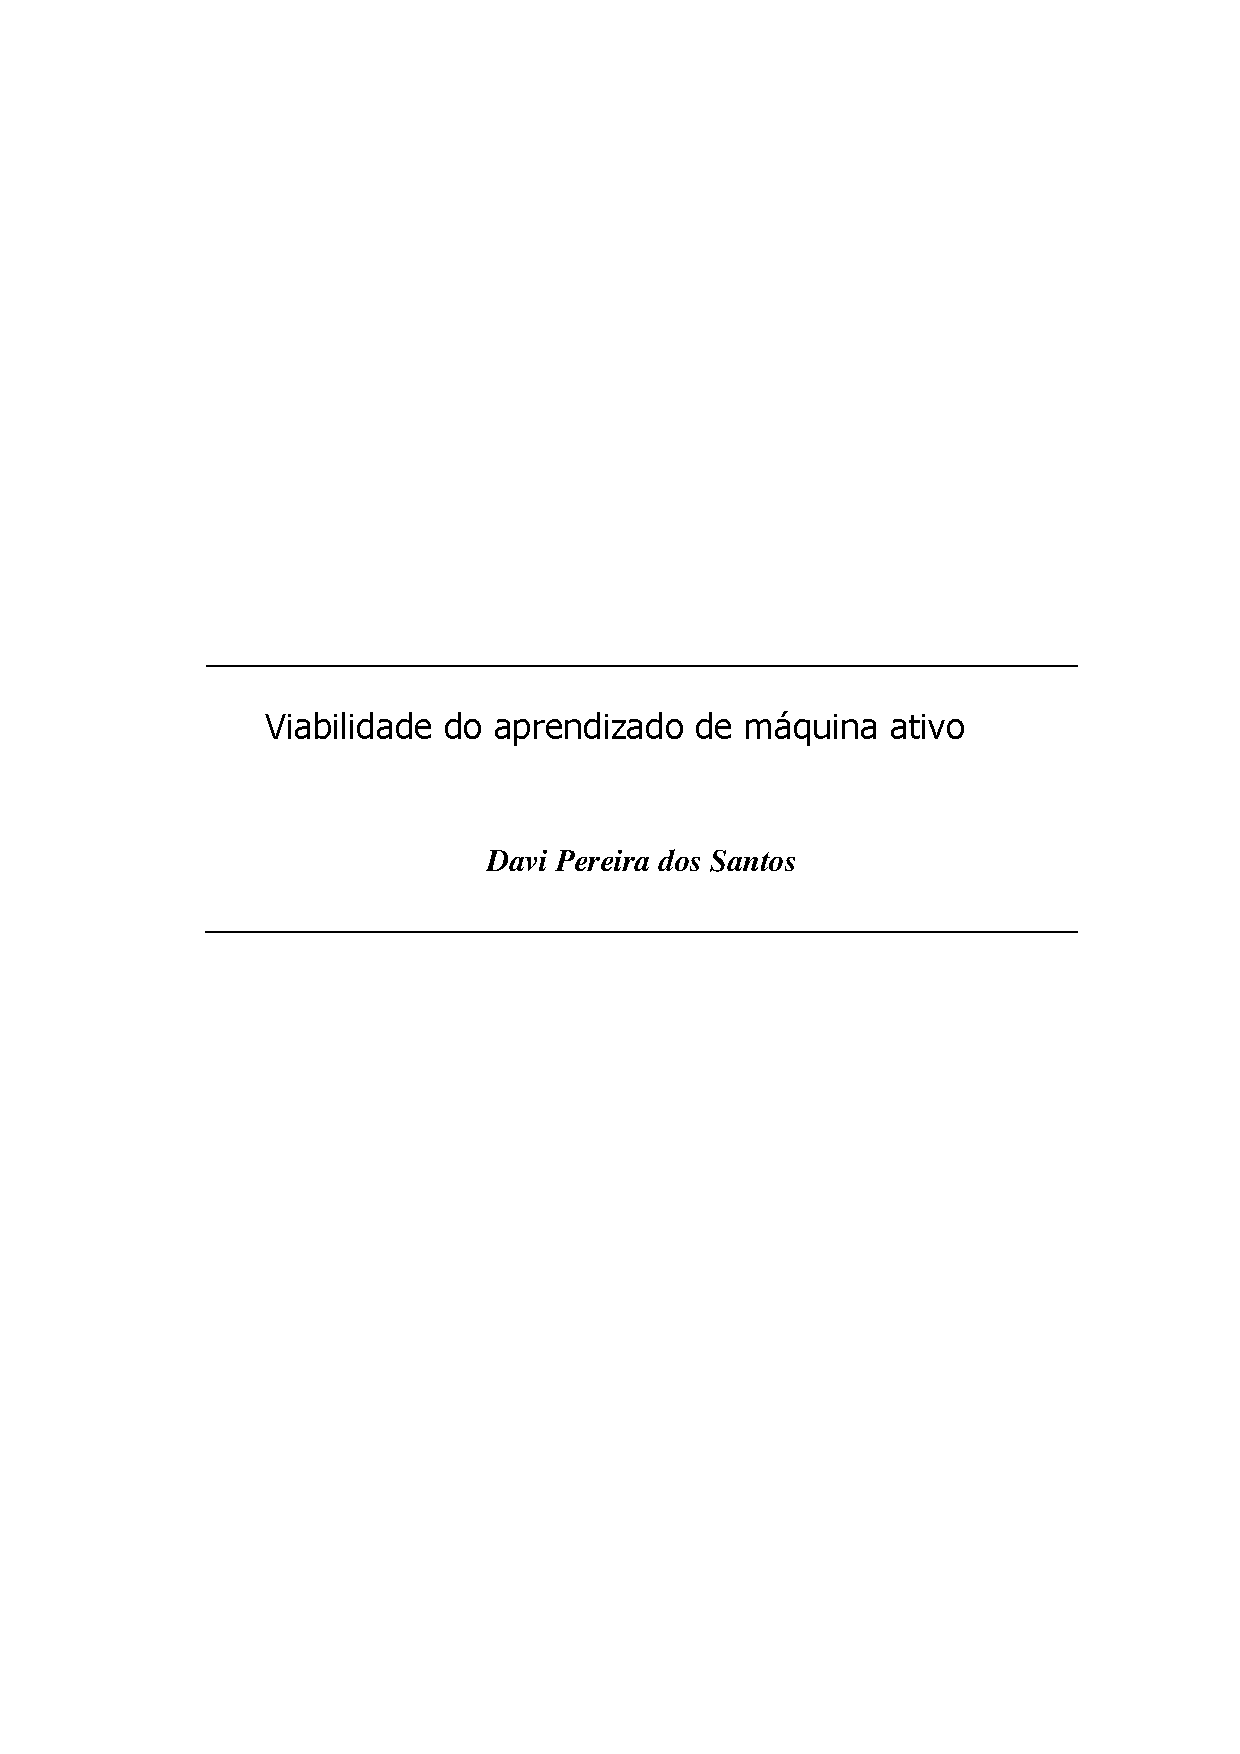
\includepdf[scale=1.06]{SECAO-POSGRAD_87_Modelo_Capa_DO_CCMC_ORIGINAL1.pdf}
  \cleardoublepage
  \newpage
  \clearpage
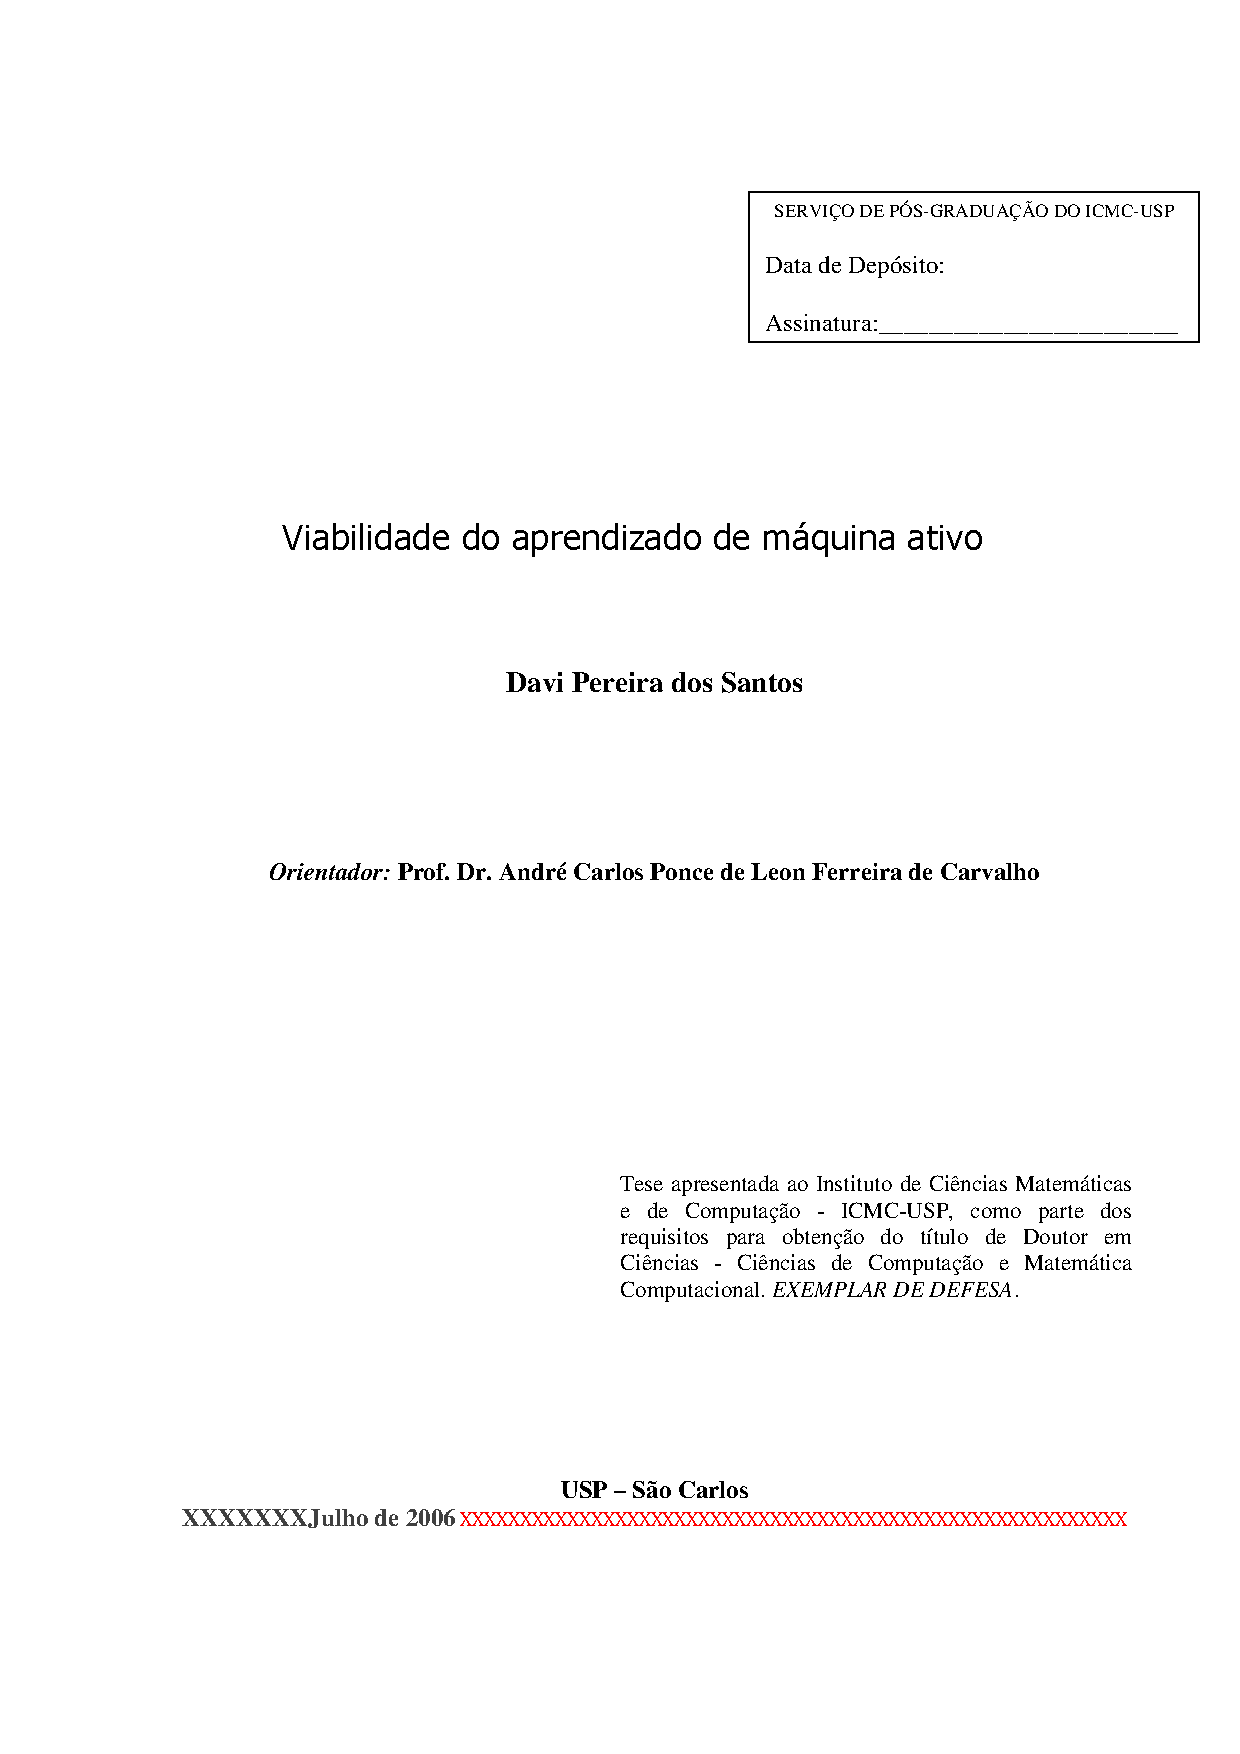
\includepdf[scale=1.06]{SECAO-POSGRAD_87_Modelo_Capa_DO_CCMC_ORIGINAL2.pdf}
\cleardoublepage
\end{titlepage}
\tikzexternalenable
\pagestyle{plain}
\onehalfspacing
\chapter*{Resumo}
Apesar do crescente avan�o no desenvolvimento de algoritmos capazes de induzir modelos preditivos
numa grande diversidade de dom�nios, entraves de cunho econ�mico, dentre outros, ainda persistem.
Embora tais modelos sejam constru�dos sem programa��o expl�cita,
eles n�o podem, em geral, dispensar a supervis�o humana no processo inicial de descoberta de r�tulos que
normalmente se atribuem a certas parcelas dos dados dispon�veis.
Em vista da forte possibilidade dos dados serem massivos,
as parcelas n�o podem ser proporcionais ao total de dados.
Elas devem permanecer pequenas, dentro do devido or�amento.
Isso prop�e um compromisso entre o custo de rotula��o e a acur�cia preditiva,
cuja solu��o pode ser a ado��o de uma t�cnica de aprendizado ativo.

Existem diversas abordagens de se amostrarem ativamente os dados para rotula��o.
Diferentemente do aprendizado passivo, n�o � poss�vel test�-las para posterior escolha da melhor
segundo alguma m�trica de acur�cia.
A cada r�tulo obtido incorre-se em custo adicional.
Dessa forma, a situa��o ideal seria a ci�ncia pr�via da melhor estrat�gia
para o dom�nio em quest�o, mesmo com poucos r�tulos conhecidos de antem�o;
ou, em maior detalhe,
para cada instante durante a aquisi��o de r�tulos naquele dom�nio.

Nesta tese, a viabilidade do aprendizado ativo � comprovada empiricamente com solidez estat�stica 
de acordo com tr�s pontos de vista: adapta��o e compara��o dos principais paradigmas e de sua efetividade em geral;
na defini��o de nichos adequados para cada estrat�gia;
e, na demonstra��o de que � poss�vel definir previamente as estrat�gias mais adequadas,
especialmente se for adotado uma chaveamento ao longo do processo de rotula��o.
� tamb�m empreendida uma an�lise amplamente negligenciada pela literatura da �rea:
o risco devido � variabilidade dos algoritmos.

% o vi�s de amostragem tem seus perigos, ent�o quando n�o h� diferen�a estat�stica entre aleat�rio e AA, deve-se prefirir aleat�rio,
% ou melhor, cluster-based, por suas garantias estatisticas peculiares.

\newpage
\thispagestyle{empty}
\mbox{}
\cleardoublepage

\tableofcontents
\cleardoublepage

\listoffigures
\addcontentsline{toc}{section}{Lista de Figuras}
\cleardoublepage

\listoftables
\addcontentsline{toc}{section}{Lista de Tabelas}
\cleardoublepage

\chapter*{Abreviaturas}
\addcontentsline{toc}{section}{Abreviaturas} %ver comando do rigolin para criar links e outras
\begin{acronym}
\acro{SMOOTE}{Synthetic Minority Over-sampling TEchnique} \acro{QoS }{Quality of Service}
\acro{DDM}{\textit{Drift Detection Method}}
\acro{AWE}{\textit{Drift Detection Method}}
\acro{SEA}{\textit{Streaming Ensemble Algorithm}}
\end{acronym}
\cleardoublepage

\listofalgorithms
\addcontentsline{toc}{section}{Lista de Algoritmos}
\cleardoublepage

\hypersetup{pageanchor=true}
\pagenumbering{arabic}
\pagestyle{fancy}
\renewcommand{\chaptermark}[1]{\markboth{\thechapter \ #1}{}}
\renewcommand{\sectionmark}[1]{\markright{\thesection \ #1}}

%Capitulos
\chapter{Introdução} \label{cap:intro}
Atualmente, o aprendizado de máquina permeia o cotidiano humano
provendo auxílio em tarefas diversas.
\ano{citar algumas(gps,digitação,fala))? precisa de ref?}
Seu bom desempenho, na tarefa de classificação, depende da existência de:
\begin{itemize}
 \item \textbf{amostragem} de dados de qualidade para construção de um acervo \ano{acervo?};
 \item um processo de \textbf{categorização} desses dados que exponha conhecimento
 suficiente para a tarefa desejada; e,
 \item um algoritmo de \textbf{aprendizado} adequado.
\end{itemize}
Enquanto a \textit{categorização} dos dados é normalmente
realizada por um supervisor humano que atribui categorias/classes para cada objeto/exemplo
de interesse contido nos dados,
a forma de \textit{amostragem} de exemplos
e a determinação do algoritmo de \textit{aprendizado} dependem de
um segundo especialista,
com conhecimento específico da área de aprendizado de máquina.

\ano{citar problemas? fadiga ...}

O segundo especialista pode resolver o problema da escolha do algoritmo
recorrendo à sua experiência pessoal ou adotando algum sistema automático de
recomendação como o \textit{meta-aprendizado} conforme descrito no
Capítulo \ref{meta}.
Ambas as abordagens, manual e automática,
são aplicáveis apenas no cenário em que o acervo, chamado de conjunto de treinamento,
já está construído.
Consequentemente, a escolha do processo de amostragem,
denominado \textit{aprendizado ativo},
precede a determinação do algoritmo de aprendizado.
\ano{isso contradiz o cenário em que o aprendiz é definido de antemão,
que é parte dos experimentos}

Da mesma forma que existe o problema da escolha do algoritmo de aprendizado
mais apropriado, existe o problema da escolha da melhor estratégia de
aprendizado ativo.
O segundo problema é mais complexo, tendo-se em vista que o sucesso
da estratégia escolhida só pode ser determinado após ter-se incorrido
em custos financeiros com a atividade de supervisão - que é realizada
frequentemente por um humano, chamado genericamente de \textit{oráculo}.
% Está implícita na seleção de dados de qualidade a economia em tempo de processamento e
% de supervisão, dado que apenas a parcela reduzida de exemplos mais relevantes
% é enviada para a análise do oráculo e processada pelo algoritmo de aprendizado.
% Como agravante, a quantidade global de dados duplica a cada dois anos
% \citep{journals/sigkdd/ZliobaiteBGGGMM12}, apontando
% para uma tendência que torna intratável a supervisão e aprendizado exaustivos
% em muitas aplicações.
% 
% Por outro lado, aplicações em que o oráculo é um processo químico, por exemplo,
% envolvem consumo de material ou a destruição dos exemplos consultados.
% Apesar de não envolver a manutenção dispendiosa de um oráculo humano
% e possivelmente não requerer uma filtragem massiva de exemplos,
% cada consulta tem um custo associado.
Dessa forma, é preciso adotar uma estratégia
com base em previsões de desempenho ou de acordo com características da base
de dados.
Na prática, essa escolha tem sido quase arbitrária, tendendo a se concentrar
no uso da estratégia mais simples (amostragem por incerteza).
Essa preferência foi reportada numa competição de aprendizado ativo,
onde também prevaleceu a ausência de estratégias possivelmente mais efetivas
como as baseadas em densidade conforme
Figura \ref{compet}.
\ano{é mesmo mais efetiva? por quê?}
\begin{figure}
\caption{Frequência de uso de estratégias na competição de aprendizado ativo
(alguns participantes adotaram mais de uma estratégia).
\textit{Adaptado de \citep{journals/jmlr/GuyonCDL11}.}}
\label{compet}
\begin{center}
    \begin{tikzpicture}
\begin{axis}[
    xbar,
%     xmin=0.0,
%     width=12cm,
%     height=40cm,
%     enlarge x limits={rel=0.13,upper},
    ytick={1,2,3,4,5,6,7},
    yticklabels={
    {amostragem por incerteza},
    {amostragem aleatória},
    {consulta por comitê},
    {aprendizado passivo},
    {redução do erro esperado},
    {mudança esperada no modelo},
    {outras}
    },
%         enlarge y limits=0.4,
    xlabel={participantes (\%)},
    ytick=data,
    nodes near coords,
    nodes near coords align=horizontal
]
\addplot [draw=black, fill=cyan!40!black] coordinates {
    (80,7)
    (42,6)
    (38,5)
    (20,4)
    (10,3)
    (5,2)
    (25,1)
};
\end{axis}
\end{tikzpicture}
\end{center}
\end{figure}

% challenge:
% global_score = (ALC-Arand)/(Amax-Arand)       Amax = 1
% semi-supervised learning is needed to achieve good performance in the first part of the learning curve
% (usar ou não semisupervised é um problema à parte, que faz parter do learner, não da estratégia; classificadores semisupervisionados são melhores, mas não é isso que se está avaliando quando se comparam estratégias; ensembles, feature selection e SMOTE também ajudam e nem por isso precisam ser empregados na comparação de estratégias)


Em consonância com esse panorama,
está a ausência de estudos comparativos
abrangentes que possam guiar o especialista na fase de amostragem.
% - até onde o conhecimento do autor permite dizer - 
\ano{AL é uma área com enfoque prático, pois visa diretamente a redução de custos.
Provavelmente por esse motivo, a pesquisa em AL é normalmente direcionada a
aplicações específicas e não a experimentos comparativos abrangentes.}


\esb{comenta possiveis deficiencias ou
lacunas das estrategias existentes (pensando nas que vou propor),
apresenta melhorias propostas;
apresenta recomendação de classificador e/ou estratégia;
apresenta hipóteses principal e secundárias.
Falar ainda dos objetivos da tese, que estao bem ligados as hipoteses}

Hipóteses secundárias
Estratégias baseadas em densidade são viáveis \ano{muito fraca essa palavra?} sem um aprendiz
objetivo: contornar o problema de escolha do algoritmo de aprendizado antes
da obtenção dos rótulos (transformando uma estratégia eficaz em agnóstica)

É possível definir a estratégia mais adequada \ano{muito forte essas duas palavras?} por meio de recomendação automática
objetivo: resolver o problema de escolha da estratégia quando o algoritmo de
aprendizado é dado previamente pela aplicação (com recomendação automática)




\section{Contribuição}\label{contribuicao}
\esb{cita os artigos/software publicados e submetidos; menciona
metodologia, compara com Everton e de que forma organiza a área}

\section{Cenário}\label{cenario}
Existem três principais cenários na literatura de aprendizado ativo
\citep{settles2010active}:
\textit{síntese de consulta por associação} ou
\ing{consulta de exemplos sintetizados}{membership query synthesis};
\ing{amostragem baseada em \pool}{pool-based sampling}; e
\ing{amostragem seletiva baseada em fluxo}{stream-based selective sampling}.
Mais detalhes são apresentados no Apêndice \ref{cenarios}.
O cenário adotado neste trabalho é baseado em \pool.
Especificamente, há as seguintes restrições de escopo:
\begin{itemize}
 \item consulta pela classe (não por valores de atributos, por exemplo);
 \item monorrótulo;
 \item distribuição estacionária;
 \item custo por erro de classificação uniforme;
 \item custo por consulta uniforme;
 \item oráculo único e constante sujeito a ruído;
 \item os domínios dos atributos nominais são previamente conhecidos;
 \item atributos sem valores faltantes;
 \item consulta \ing{um a um}{on-line}.
\end{itemize}

\section{Estrutura do documento}\label{estrutura}
O contexto da pesquisa, a notação matemática e a terminologia adotadas e a revisão da literatura das áreas
envolvidas neste trabalho são apresentados no Capítulo \ref{contexto}.
No Capítulo \ref{propostas},
são apresentadas as propostas de algoritmos.
O Capítulo \ref{metodologia} contém os métodos de avaliação e detalhes de
implementação comuns a todos os experimentos descritos neste documento.
Essa avaliação empírica e seus resultados associados são apresentados
no Capítulo \ref{experimentos}.
Adicionalmente, uma abordagem baseada em meta-aprendizado
é proposta e avaliada no Capítulo \ref{aml}.
Por fim, uma análise geral unificada das contribuições da tese e
desdobramentos futuros são apresentados no
Capítulo \ref{conclusao}.
Detalhes sobre os cenários de aprendizado ativo, resultados,
formatação, estilo e terminologia podem ser encontrados nos apêndices \ano{ <- revisar}.

\ano{mencionar apendice de rev. sistemática? outros aps?}

%
% No Capítulo \ref{cap:classificacao}, é apresentada a notação utilizada neste trabalho juntamente com um texto introdutório sobre aprendizado supervisionado para contextualizar as duas revisões bibliográficas que o seguem: a primeira sobre \textit{ensembles} e a segunda sobre \textit{fluxos de dados}.
% Ao final, \textit{ensembles} voltados especificamente a fluxos de dados são revisados.
%
% No Capítulo \ref{cap:aprendizado-ativo}, o \textit{aprendizado ativo} é descrito em detalhes a respeito dos cenários mais comuns e das estratégias normalmente adotadas.
% Os trabalhos recentes nos quais se baseia diretamente a linha investigativa adotada são explicitados na Seção \ref{sec:panorama}.
%
% O plano de trabalho é apresentado no Capítulo \ref{cap:plano} e contempla a situação atual do aluno no programa de doutorado, os recursos disponíveis, as hipóteses formuladas, a metodologia e o cronograma.
%
% Finalmente, no Capítulo \ref{cap:experimentos}, são mostrados experimentos ilustrativos da mudança de conceito e da diversidade de comportamento entre diferentes classificadores. %overview AL, (ELM?)
% % \include{al} %estrats, experimentos de exemplo, limita��es (que vou superar)
% % \newpage
\newpage

\section{M�quinas Extremas}\label{elmorig}
Até onde o conhecimento dos autores permite alcançar,
não existe pesquisa em aprendizado ativo que enfoque ELMs.
As poucas abordagens encontradas usam AA apenas como uma ferramenta
sem maiores desenvolvimentos em torno do AA em si.
Um exemplo é o \textit{standard deviation query-by-bagging} \cite{conf/his/AyerdiMG12},
que � conceitualmente pr�ximo � \textit{amostragem por incerteza}
e \textit{Query-by-Committee}.
É uma abordagem genérica no sentido de que ela pode ser aplicada em
um \textit{ensemble} de modelos gerados por qualquer  algoritmo de aprendizado.
Outro exemplo é o \textit{fixation-based active learning},
que treina uma ELM para ser usada como uma tabela de mapeamento de cores
(\textit{color look-up table}) para segmentação.
Na parte de AA, é calculada a entropia de um histograma feito das intensidades
em uma região circular \cite{journals/soco/PanPLW12}.
Novamente, AA é usado apenas como uma ferramenta independente do classificador adotado.
Outro, menos relacionado,
exemplo é a incerteza de um \textit{framework} bayesiano não-paramétrico baseado em ELMs \cite{conf/ictai/ChatzisKD11}.
À parte desses trabalhos isolados, nenhum estudo comparativo abrangente foi encontrado na literatura de aprendizado de máquina.

% von Zuben:
% ftp://ftp.dca.fee.unicamp.br/pub/docs/vonzuben/ia353_1s13/topico4_P4_1s2013_view.pdf
% Ele coloca uma coluna adicional de 1s em H.
% Considerando que a matriz H tenha posto completo
Uma \ing{\elm}{Extreme Learning Machine} (ELM) � uma rede, n�o
necessariamente neural e com treinamento diferenciado, que tem recebido crescente
aten��o devido � sua simplicidade e performance, compar�vel com o estado da arte
em classifica��o \citep{journals/tsmc/HuangZDZ12}.

When one needs prompt response from machine learning systems
or has massive data to process in an acceptable time,
it is necessary to resort to fast classifiers.
One such classifier is the Extreme Learning Machine (ELM).

Sua topologia � a mesma de um \ing{Perceptron multicamadas}{MultiLayer Perceptron} - MLP
\citep{haykin2004comprehensive}, mas com a quantidade de camadas ocultas fixada em apenas uma.
Essa topologia � chamada de \ing{rede de camada oculta �nica com direcionamento entrada-sa�da}
{Single Hidden Layer Feedforward Network}
(SLFN).
Com rela��o � configura��o dos neur�nios, a ELM � desprovida do peso de vi�s na
camada de sa�da e aceita fun��es de ativa��o n�o diferenci�veis na camada oculta.
A camada oculta � gerada com pesos aleat�rios e mantida sem altera��es
durante o treinamento.
Essa ideia remonta ao trabalho de \cite{rosenblatt1961principles} que optou
por ajustar apenas as �ltimas camadas.
Na ELM, o ajuste tira proveito do fato de que a camada de sa�da
� um modelo de regress�o linear.
Esse tipo de modelo tem sido estudado desde o s�culo XIX \citep{legendre1805nouvelles},
logo possui uma vasta literatura de m�todos que permitem alterar a rede de
forma otimizada conforme explorado a seguir e nas se��es
\ref{press}, \ref{emelm} e \ref{oselm}.

A ELM enquanto conceito existe desde o trabalho de \cite{journals/tnn/HuangB98}
onde � proposta a busca direta pelo valor dos pesos de sa�da sem a necessidade de itera��es
e o uso de qualquer fun��o de ativa��o limitada n�o linear.
Neste trabalho, dentre os dois tipos de n� mais frequentemente usados,
aditivo log�stico sigmoide e fun��o de base radial \citep{journals/tsmc/HuangZDZ12},
optou-se pelo primeiro.
Assim, a fun��o preditiva de uma SLFN com $L$ neur�nios ocultos pode ser representada
como segue na Equa��o \ref{eqelm}.
\begin{equation} \label{eqelm}
f(\bm{x}_{(t)})= \argmax_{\bm{y} \in Y}{\displaystyle\mathop{\sum} _{l=1}^{L}\beta_{l,c(\bm{y})}
g(\bm{a}_l \bm{x}_{(t)} + b_l)} = \bm{y}_{(t)}
\end{equation}
% }, \quad j=1, \cdots, {\it N}.

$\beta_{l,o}$ � o peso da sinapse que conecta o neur�nio oculto $l$ ao neur�nio de sa�da $o$;
$c(\bm{z})$ � uma fun��o auxiliar que retorna o �ndice correspondente � classe
representado pelo vetor $\bm{z} \in Y$;
$g$ �, neste trabalho, a fun��o sigmoide log�stica;
$\bm{w}_l$ � o vetor de pesos do neur�nio $l$ com cada valor $w_i$ representando o peso entre a
entrada $i$ e o neur�nio $l$ e, sendo o produto interno deste neur�nio uma equa��o de reta no
espa�o de par�metros, $b_l$ � o valor de seu vi�s de deslocamento em rela��o � origem.
Mais detalhes da formula��o da primeira camada podem ser consultados na literatura sobre o
Perceptron multicamadas convencional \citep{haykin2004comprehensive}.
Se $\beta$ for adotada como uma matriz, a equa��o \ref{eqelm} pode ser escrita compactamente da
forma (Equa��o \ref{eq2}):
\begin{equation} \label{eq2}
H \beta = T
\end{equation}

onde $H$ � a \ing{matriz de sa�das da camada oculta}{hidden layer output matrix} da SLFN,
ou seja, cada coluna corresponde � sa�da de um neur�nio oculto e cada linha corresponde a um
exemplo do conjunto de treinamento;
$\beta$ � a matriz contendo os pesos que conectam a camada oculta � camada de sa�da, ou seja, cada
coluna corresponde a um neur�nio de sa�da e cada linha corresponde a um neur�nio oculto;
e $T$ � a matriz objetivo, que cont�m em cada linha a
representa��o bin�ria (um-de-n) $\bm{y}$ da classe de cada exemplo.
O c�lculo de $\beta$, que � an�logo a treinar a rede,
pode ser feito por meio do c�lculo da pseudoinversa $H^{\dagger}$ de $H$
\citep{rao1971generalized}:
\begin{equation} \label{eq3}
\beta = H^{\dagger} T
\end{equation}
Essa abordagem tem a vantagem de ser tamb�m uma minimiza��o da norma dos pesos -
propriedade que reduz a possibilidade de sobreajustamento aos dados de treinamento
\citep{journals/tit/Bartlett98}.
Uma vez calculada a pseudoinversa,
novos exemplos podem alimentar a entrada da rede e gerar predi��es conforme a fun��o $f$
presente na Equa��o \ref{eqelm}.

% https://reference.wolfram.com/mathematica/tutorial/LinearAlgebraMatrixComputations.html
% explica bem a pinv

\subsection{Topologia}


A defini��o da topologia de uma rede neural � uma tarefa complexa.
\cite{sheela2013review}, por exemplo, citam cento e uma heur�sticas para a defini��o do
n�mero de neur�nios ocultos.
No caso espec�fico da ELM, h� trabalhos que prop�em a defini��o autom�tica de $L$,
por�m com a introdu��o de um novo par�metro \citep{journals/ijon/YuHMNHSL14} ...



On Over-?tting in Model Selection and Subsequent Selection Bias
n Performance Evaluation (2010)
% http://jmlr.org/papers/volume11/cawley10a/cawley10a.pdf

Like over-?tting in training, over-?tting in model selection is likely to be most severe when
the sample of data is small and the number of hyper-parameters to be tuned is relatively large.
Likewise, assuming additional data are unavailable, potential solutions to the problem of
over-?tting the model selection criterion are likely to be similar to the tried and tested
solutions to the problem of over-?tting the training

criterion, namely regularisation (Cawley and Talbot, 2007), early stopping (Qi et al., 2004) and
model or hyper-parameter averaging (Cawley, 2006; Hall and Robinson, 2009).

Another approach is simply to avoid model selection altogether using an ensemble approach,
for example the Random Forest (RF) method

regarding leave-one-out cross-validation, Kulkarni et al. (1998) comment
In spite of the practical
importance of this estimate, relatively little is known about its properties.

Bengio and Grandvalet (2004) have shown there is no unbiased estimate of the variance
of (k-fold) cross-validation.


The task of model selection is frequently done by the application of some kind of validation,
preferably cross-validation for efficient data reuse.
Within this context,



Another approach is to adopt one of the several methods for selecting, growing and/or shrinking the ELM's topology from the literature with its own requirements:
E-ELM searches through a population of ELMs using the accuracy on a \textit{validation set} as measure of fitness \cite{journals/pr/ZhuQSH05};
% http://citeseerx.ist.psu.edu/viewdoc/download?rep=rep1&type=pdf&doi=10.1.1.217.3643
I-ELM and EI-ELM use a predefined \textit{training error} or maximum number of iterations as stopping criterion \cite{journals/tnn/HuangCS06};
OP-ELM \cite{journals/tnn/MicheSBSJL10} adopts the PRESS statistic \cite{mye:book};
HQ-OP-ELM uses the non-exact Hannan-Quinn criterion which is faster than PRESS for very large datasets \cite{conf/esann/MicheL09};
% http://research.ics.aalto.fi/eiml/Publications/Publication119.pdf
% Do mesmo autor de OP-ELM, � mais r�pido para bases muito grandes e equivalente em bases pequenas. O m�todo n�o � exato.

% EnhancedOS-ELM uses a complex set of three criteria including the Root Mean Squares value of the error over a sliding window
% (enhanced) EOS-ELM 2008
% http://ieeexplore.ieee.org/xpls/abs_all.jsp?arnumber=4597855&tag=1

% for SLFNs with RBF hidden nodes based on minimal resource allocation network (MRAN) algorithm.
% Although we can get more compact network structure using EOS-ELM in the end, the method is
% complicate and only suitable for RBF hidden nodes (texto do ceos)).

CEOS-ELM provides the optimal hidden nodes according to the \textit{expected error} given by the user \cite{conf/ijcnn/LanSH09};
% Experimentos: N0 come�a grande (abalone=75, 200, 500, 800); Lmax em torno de ? de N0;
% f�rmula 13 � central na atualiza��o de Beta pro EM-ELM.
% http://ieeexplore.ieee.org/xpls/icp.jsp?arnumber=5178608 tem latex
% http://ieeexplore.ieee.org/xpl/login.jsp?tp=&arnumber=5178608&url=http%3A%2F%2Fieeexplore.ieee.org%2Fxpls%2Fabs_all.jsp%3Farnumber%3D5178608


EM-ELM also relies on a \textit{targert error} or on the pace of its reduction \cite{journals/tnn/FengHLG09};
% http://ieeexplore.ieee.org/xpls/abs_all.jsp?arnumber=5161346&tag=1
% experimentos: sigmoide, normalizado entre [-1,1] (atts) e [0,1] (output); alguns datasets com ai��o de neur�nios de 25 em 25 e outros de 1 em 1; target accuracy arbitrariamente setada em 90%.
% Huang et al. [6] has further shown that if the N training data are distinct, H is column full rank with probability one when L<=N.
% In real applications, one need not request that the network output
% error E(Hk ) is less than the target error . In fact, the network growing
% procedure could stop if the network output error reduced very slowly,
% one may also apply cross-validation methods in learning of EM-ELM.
% rank H = L, ou seja, duas condi�oes de acordo com a defini��o de rank MxN mais abaixo.
% 1) L <= N0  (pois o rank � sempre da menor dimens�o)
% 2) todas colunas de H s�o linearly independentes*
% http://www.cds.caltech.edu/~murray/amwiki/index.php/FAQ:_What_does_it_mean_for_a_non-square_matrix_to_be_full_rank%3F
% So if there are more rows than columns (), then the matrix is full rank if the matrix is full column rank.
% Full-rank MxN = full [column|row] rank = todos independentes = [M|N]



% EnsembleOS-ELM
CS-ELM depends on the \textit{training Mean Squared Error} \cite{journals/ijon/LanSH10a};
TS-ELM relies on the final prediction error criterion which compromises the \textit{validation error} and $L$ \cite{journals/ijon/LanSH10};
% http://www.sciencedirect.com/science/article/pii/S0925231210003401
% http://ieeexplore.ieee.org/xpls/icp.jsp?arnumber=4746040
% http://download.springer.com/static/pdf/722/chp%253A10.1007%252F978-3-642-14922-1_2.pdf?auth66=1393101679_7d2915b6efac3e939585e1273dab21f4&ext=.pdf

ELM-TV requires a predefined \textit{expected error} \cite{conf/apccas/CingolaniSP08};
DT-ELM adjusts $L$ automatically, but depends on a new parameter, the number of clusters \cite{journals/ijon/YuHMNHSL14};
AIE-ELM requires the definition of the \textit{expected learning accuracy} \cite{conf/ais2/ZhangLHS11};
AG-ELM selects the neurons that achieve the \textit{best generalization performance} \cite{journals/tnn/ZhangLHX12};
% http://ieeexplore.ieee.org/xpls/abs_all.jsp?arnumber=6125249

D-ELM (a vers�o HTML tem os TEX sources das f�rmulas da ELM) 2013
Dynamic Extreme Learning Machine and Its Approximation Capability
http://ieeexplore.ieee.org/xpls/icp.jsp?arnumber=6459569
The key idea of D-ELM is the following. The network starts with one random hidden unit. Then, at each subsequent step, several new networks with different numbers of hidden nodes are first generated. Among all these new networks and the network obtained at the previous step, the generalization performance will be compared, and the ?best? one, whose number of hidden nodes is the least among those having the best generalization, will be selected. Adding one more random hidden node to such selected network then results in the network for the current step. In D-ELM, the hidden nodes are randomly generated, and the output weights are updated incrementally by using the error-minimization-based method proposed in [6].
...
Comparing with those constructive ELMs, AG-ELM has two features: 1) the hidden-node number of AG-ELM is determined in an adaptive way in the sense that the existing networks may be replaced by some newly generated networks with better performance rather than always keeping those existing ones; 2) a group of new networks are generated at each step in AG-ELM (i.e.,  networks with different numbers of hidden nodes are generated at the th step), while in other constructive ELMs, only one new network is generated at each step.

Comparativo com 10 variantes de ELM 2013, citar pra dizer que existem elms pra outras finalidades
Extreme learning machine and its applications

% % % OPIUM (Online PseudoInverse Update Method) 2013
% % % Learning the pseudoinverse solution to network weights
% % % http://www.sciencedirect.com/science/article/pii/S089360801300049X
% % % ?
% % % We present an online or incremental method of computing the pseudoinverse precisely, which we argue is biologically plausible as a learning method, and which can be made adaptable for non-stationary data streams. The method is significantly more memory-efficient than the conventional computation of pseudoinverses by singular value decomposition.
% % % ?
% % % Neural Engineering Framework ( Eliasmith & Anderson, 2003) in computational neuroscience and the Extreme Learning Machine (ELM) ( Huang, Zhu, & Siew, 2006) in the machine learning field, both synthesize three-layer feedforward networks which are superficially similar to the classic multilayer perceptron ... What makes these architectures unique is that the input layer signals are connected to an unusually large number of hidden layer neurons, using randomly initialized connection weights. This has the effect of randomly spreading or projecting the inputs from their original input dimensionality to a hidden layer of very much higher dimensionality. It is then possible to find a hyperplane in the higher dimensional space which approximates a desired function regression solution, or represents a classification boundary for the input?output relationship.
% % % ?
% % % We will refer broadly to this class of methods as linear solutions to higher dimensional interlayer networks (LSHDI).
% % % ?
% % % structures embodying the LSHDI principle may exist in the brain. For example, recent work by Rigotti, Ben Dayan Rubin, Wang, and Fusi (2010) in modeling recorded cortical activity in monkeys performing context-sensitive tasks shows that complex rule-based tasks require both sensory stimuli and internal representation of states; and that a significant number of random connections placed between input sources and a hidden interlayer, and random recurrent connections between interlayer neurons, are necessary for optimal performance. They describe these interlayer neurons as generating mixed selectivity, which is equivalent to increasing the dimensionality of the state representation.
% % % ?
% % % An obstruction to acceptance of the LSHDI method as being biologically plausible is the necessity to compute the pseudoinverse of a matrix.
% % % ?
% % % The solution to the network weights is exactly the same as that which would be calculated by singular value decomposition. It converges with a single forward iteration per input data sample, and as such is ideal for real-time online computation of the pseudoinverse solution.
% % % ?
% % %  It requires significantly less memory than the SVD method, as its memory requirement scales as the square of the size of the hidden layer, whereas the SVD memory requirement scales with the product of the hidden layer size and the size of the training data set.
% % % ?
% % % OPIUM is adapted from an iterative method for computing the pseudoinverse, known as Greville?s method (Greville, 1960).
% % % ?
% % % Pseudoinverse methods were widely used in an earlier era of neural network research, to the extent that a significant class of Kohonen-type linear associative memories were known as pseudoinverse neural networks (PINNs) (Kohonen, 1988 and Kohonen, 1989). The key variations in the LSHDI use of the method are in the initial spreading to higher dimension, and the associated nonlinear activation performed on the higher dimension signals.
% % % ?
% % %  typical test error on the raw MNIST data set is 2.75%
% % % ?
% % % apart from the number of hidden-layer neurons, there are no parameters to be tuned


Fast sparse approximation of extreme learning machine(2014)
http://www.sciencedirect.com/science/article/pii/S0925231213010047
the solution of LS-SVM lacks sparseness and hence, the test speed is significantly slower than that of other algorithms, such as the support vector machine (SVM) [5] and [6] and neural networks
?
ELM: unified learning mode for regression, binary, and multiclass classification
?
aparentemente somente para kernels (talvez seja um restri��o inerente � tarefa de se criar uma ?sparse solution?.
?
The popular Gaussian kernel function K(u,v)=exp(??2?u?v?) is used in SVM, LS-SVM, SLFN-ELM, and FSA-ELM. In order to achieve a good generalization performance, the cost parameter C and kernel parameter ? of SVM, LS-SVM, and SLFN-ELM, need to be chosen appropriately.


TOSELM: Timeliness Online Sequential Extreme Learning Machine 2014
http://www.sciencedirect.com/science/article/pii/S0925231213009120
Timeliness here means the data distribution or the data trend changes with time passing by.



Parsimonious Extreme Learning Machine Using Recursive Orthogonal Least Squares (2014):
% http://ieeexplore.ieee.org/stamp/stamp.jsp?tp=&arnumber=6704311
Casta�o et al. [17]
proposed a robust and pruned ELM approach based on prin-
cipal component analysis (PCA), termed PCA-ELM, whereby
the PCA method is used to select the hidden nodes from input
features while corresponding input weights are deterministi-
cally defined as principal components rather than random ones.
Note that the deterministic approach to hidden node selection
inevitably results in poor accuracy especially for noisy data.
% http://en.wikipedia.org/wiki/Multicollinearity#Remedies_for_multicollinearity :
Note that one technique that does not work in offsetting the effects of multicollinearity is orthogonalizing the explanatory variables (linearly transforming them so that the transformed variables are uncorrelated with each other): By the Frisch?Waugh?Lovell theorem, using projection matrices to make the explanatory variables orthogonal to each other will lead to the same results as running the regression with all non-orthogonal explanators included.





Comparando com SVM (2012:
% http://www.ntu.edu.sg/home/egbhuang/pdf/ELM-Unified-Learning.pdf
% http://citeseerx.ist.psu.edu/viewdoc/download?doi=10.1.1.298.1213&rep=rep1&type=pdf
% ELM tends to have better scalability and achieve similar (for regression and
% binary class cases) or much better (for multiclass cases) generaliza-
% tion performance at much faster learning speed (up to thousands
% times) than traditional SVM and LS-SVM.
% ...
% According to the ridge regression theory [37], one can add
% a positive value to the diagonal of HT H or HHT ; the resul-
% tant solution is stabler and tends to have better generalization
% performance. Toh [22] and Deng et al. [21] have studied the
% performance of ELM with this enhancement under the Sigmoid
% additive type of SLFNs.
% ...
% In this specific case, similar to SVM, LS-SVM, and PSVM,
% the feature mapping h(x) need not be known to users;
% instead, its corresponding kernel K(u, v) (e.g., K(u, v) =
% exp(?? u ? v 2 )) is given to users. The dimensionality L of
% the feature space (number of hidden nodes) need not be given
% either.


% Architecture selection for networks trained with extreme learning machine using localized generalization error model 2013
% http://www.sciencedirect.com/science/article/pii/S0925231212004328
% s� pra RBF.
% If the number of hidden nodes is equal to the number of distinct training samples, the matrix H is square and invertible, and SLFNs can approximate these training samples with zero error.



% multi-objective micro genetic ELM (?G-ELM) 2013:
% http://www.sciencedirect.com/science/article/pii/S0925231213000520
% ?
% EI-ELM and EOS-ELM are the least competitive
% ?
% Regarding the error of OP-ELM and OS-ELM, our algorithms beat them in 15 and 14 problems, or in 20 and 16 if we consider the cases in which they show an unstable behavior.
% ?
% hidden nodes, we obtain a lower number than ELM in 22 out of 26 problems  and lower than BP in 13.
% ?
% BP exhibits a very stable behavior, but its execution time is very high compared to the other algorithms, see Fig. 4.
% ?
% Sobre a busca dos parametros �timos: we consider that the relationship is parabolic and we test the significance of its quadratic term
% ?
% n�o aparenta ser incremental (on-line)

$\mu$G-ELM also depends on the \textit{mean square error} \cite{journals/ijon/LahozLM13};
D-ELM depends on the \textit{generalization performance} \cite{journals/tcyb/ZhangLHXS13};
FSA-ELM changes $L$ indirectly by an additional parameter \cite{journals/ijon/LiMJ14};

optimal pruning OP-ELM (2010):
http://research.ics.aalto.fi/eiml/Publications/Publication157.pdf
Rong et al. [9]presented a pruned ELM (P-ELM). It starts with a large network and then eliminates the hidden nodes that have low relevance to the class labels by using statistical criteria, namely the Chi-squared
OP-ELM methodology has three steps: (1) Build the SLFN using the original ELM algorithm, (2) Rank the hidden nodes by applying multi-response sparse regression algorithm (MRSR) [11], (3) Select the hidden nodes through leave-one-out

There is one SVM-based approach in which $L$ is not critical,
but it is outside the scope of this paper \cite{conf/esann/FrenayV10}.


Leave-One-Out (LOO) is the least biased estimator \cite{conf/ijcai/95}
and usually the most computationally expensive.


a unica vantagem que varias das variacoes da ELM promove eh,
por exemplo, adicionar um neuronio sem precisar retreinar a rede toda.
ainda assim, elas dependem de uma estimativa boa do erro para decidir se continua crescendo.


Another approach is to explore the fact that $L$ is dataset-dependent.
It is possible to use \textit{meta-learning} to discover the relations between meta-attributes and $L$.
This was proposed recently in the literature,
with $L$ in the range $[1,300]$ for 93 regression problems \cite{conf/cbic/lucas11}.
An already trained meta-classifier can be used to perform a warm start,
limiting the search space for model selection.
However,
both this step of refining the search and the very expensive previous step of training the meta-classifier require an efficient and immune-to-overfitting validation process.

citar exemplo de evolutionary ELM



EM-ELM eh mais apropriado aqui do que CEOS-ELM, pois o treinamento eh num lote soh.
a OS-ELM serve apenas para os decrementos.
EM-ELM poderia ser usado para acelerar ambos LLOOE and LOO,
mas no caso do LOO seria preciso manter N modelos em mem�ria durante todo o processo.

CEOS-ELM addresses both the weights incremental update due to new instances arrival and the adequate growing of the hidden layer.
However, from the original paper,
it is possible to note that the convergence (to the original ELM) requires a certain amount of instances for the initial training.
Apparently, the advantage of CEOS-ELM is to reduce training time in large training sets
by avoiding recalculation of the pseudo-inverse of H from scratch at every time step.

se CEOS comecar a partir de $L=1$, entao eh aplicavel a model selection (soh em batch learning por eventuais problemas de convergencia quando se comeca com poucos exemplos).

Like in the other ELM variants,
it is impossible to determine the target accuracy nor to define confidently $L_0$, $L_{max}$ and $N_0$ beforehand.
Also, $L_{max}$ is around a third of $N_0$ which is impossible for small $N_0$s.



Several fast cross-validation techniques have been proposed in the literature for different classifiers.
Least-Squares Support Vector Machines leave-one-out in linear time complexity
\cite{journals/nn/CawleyT04}.
Classifiers whose model space forms a monoid or a group and whose batch trainer is a
homomorphism \cite{conf/icml/Izbicki13}.
ELM-FLOO has time complexity $mathcal{O}(n)$ \cite{xue2011fast}.

Some classifiers can be trivially used for incremental/decremental learning, e.g. Naive Bayes  (NB) and 5-NN \cite{conf/ecml/Lewis98,journals/tit/Hart68}
C4.5 and Very Fast Decision Trees (VFDT) \cite{books/mk/Quinlan93,conf/kdd/DomingosH00} it is not trivial.

%software/algorithms/hardware
The library Matrix-Toolkits-Java was used to  interface the reference implementation of LAPACK with Debian default compilation.
%reference implementation of LAPACK para evitar instabilidade numerica (= matriz singular ocorrer muito cedo)
Intel(R) Core(TM) i7-3630QM CPU @ 2.40GHz




% http://research.ics.aalto.fi/eiml/Publications/Publication208.pdf
% adjusts $L$ automatically, but depends on a new parameter, the number of clusters
% 
% AIE-ELM 2011
% Extreme Learning Machine with Adaptive Growth of Hidden Nodes and Incremental Updating of Output Weights
% http://link.springer.com/chapter/10.1007%2F978-3-642-21538-4_25
% AIE-ELM grows the randomly generated hidden nodes in an adaptive way in the sense that the existing hidden nodes may be replaced by some newly generated hidden nodes with better performance rather than always keeping those existing ones in other incremental ELMs. The output weights are updated incrementally in the same way of error minimized ELM (EM-ELM). Simulation results demonstrate and verify that our new approach can achieve a more compact network architecture than EM-ELM with better generalization performance.
Outros trabalhos escolhem neur�nios

\ano{pegar no gdocs as dezenas de cita��es e num artigo em que resumi varias}

Por fim, h� propostas que buscam pelos melhores pesos da camada oculta,
entretanto passa-se a se tratar de um desvio da ideia original mais pr�ximo
das redes neurais convencionais e sua complexidade de configura��o do que
da simplicidade da ELM original.
Fixado o tipo de n�, os �nicos par�metros a ajustar a quantidade de neur�nios na camada oculta
e os valores de suas conex�es sin�pticas.
Dada uma fun��o geradora de pesos aleat�rios ou pseudoaleat�rios e sua semente geradora,
a quantidade de
neur�nios $L$ na camada oculta pode ser vista como o �nico par�metro a se ajustar.
Entretanto, h� evid�ncias de que a proje��o no espa�o de maior dimensionalidade
realizada pela camada oculta aleat�ria � inferior � realizada por uma MLP,
por exemplo (\citep{parviainen2011studies}).
% https://aaltodoc.aalto.fi/bitstream/handle/123456789/5067/isbn9789526043128.pdf?sequence=1
% The only theoretically motivated upper limit for the number of hidden units to try is N (which is enough for zero training error).
% ...
% At that limit, computing pseudoinverse corresponds to ordinary inversion of an N � N matrix, with a complexity of O(N3). In practice, smaller upper limits are used.
% ...
% Aqui tem uns desenhos legais mostrando que a proje��o aleat�ria da ELM
% no espa�o de maior dimens�o � algo que pode ser melhorado na p�gina 47.

Esse par�metro frequentemente n�o � cr�tico \citep{conf/esann/FrenayV10}.
% http://www3.ntu.edu.sg/home/EGBHuang/pdf/ELM_IJCNN2004.PDF \citep{huang2004extreme}
% simulation results in artificial and real world cases done in [7] as well as in this paper further
% demonstrated that no gain is possible by adjusting the input weights and the hidden layer biases
Apesar disso, 
,
por�m

% * A partir de um certo momento, a camada oculta passou a ser tratada como um
% conjunto de para�metros e n�o apenas seu tamanho. Da� surgiram as propostas
% evolucion�rias/evolutivas(?) em oposi��o �s propostas de crescimento da camada
% e/ou de atualiza��o dos pesos.

\subsection{PRESS}\label{press}
% Meta-learning to optimize the number of hidden nodes of MLP networks trained
% by Extreme Learning Machine algorithm (2011)
% http://www.mendeley.com/download/public/1683461/5291097694/743b3ac1a6f01b8b9ad380254dc9ee7de2146086/dl.pdf
% \citep{prud2011}

Um desses m�todos, chamado
\textit{soma dos quadrados dos erros de predi��o} - PRESS\footnote{\textit{PREdiction Sum of Squares}}
\citep{myers2000classical,allan1974relationship}, permite estimar o erro de generaliza��o do modelo.
Exceto nos casos de instabilidade num�rica, essa estimativa � exata e equivalente � que seria obtida
pela valida��o cruzada via \textit{Leave-One-Out} (LOO), representando uma redu��o na complexidade
computacional em rela��o � quantidade de treinamentos de linear para constante - ou
de quadr�tica para linear, se for considerada a quantidade de exemplos.

% http://www.jstor.org/stable/2686028?__redirected
% o come�o fala do PRESS, com formula clarificando(?)

% (see [15] and [16] for details of this formula and its implementations)
% 15:Classical and Modern Regression With Applications,
% 16:?Recursive lazy learning for modeling and control,? http://www.researchgate.net/publication/2301623_Recursive_Lazy_Learning_for_Modeling_and_Control/file/79e4151136c53c3067.pdf

.
\cite{journals/ijon/HeeswijkMOL11}, por exemplo, recalculam a pseudoinversa a cada novo neur�nio
acrescentado at� encontrar a topologia com a menor PRESS.
Eles implementaram uma ELM espec�fica para \ing{unidades de processamento gr�fico}
{Graphics Processing Unit} (GPU).
No presente trabalho, exceto para SGmulti, os conjuntos de treinamento n�o passam de $200$ exemplos,
n�o justificando o uso de GPU, especialmente em vista do custo de transfer�ncia de dados.

Quando se disp�e 

\ano{pegar pap�is com f�rmulas do press? A f�rmula via EM-ELM mais abaixo deve ser suficiente.}

Outra diferen�a � a op��o pelo crescimento incremental da
\ing{\elm por minimiza��o do erro}{Error Minimized Extreme Learning Machine} -
EM-ELM \citep{journals/tnn/FengHLG09}.
Al�m de permitir o crescimento da rede sem recalcular a pseudoinversa,
a EM-ELM permite o c�lculo da PRESS a um custo reduzido.

\ano{no artigo e em algum lugar da tese, preciso expor o algoritmo que defini para unir OS, EM e PRESS,
que � incrementar de 1 em 1 exemplo
e selecionar topologia a cada 4, testando a faixa de  de L-10 at� L+10 neur�nios;
come�ando com L=1}
% \ano{PRESS: erro estatistico (de regress�o?)}
% 
% \ano{quadrado do res�duo: erro I e CI?}
% 
% diferencia 'statistical error' e 'residual':
% 
% {http://en.wikipedia.org/wiki/Errors\_and\_residuals\_in\_statistics}
% 
% error (or disturbance) of an observed value is the deviation of the observed value from
% the (unobservable) true function value
% residual of an observed value is the difference between the observed value and the
% estimated function value.

\subsection{EM-ELM} \label{emelm}

% * EM-ELM serve de base para v�rias variantes de ELM: AIE-ELM, D-ELM, CEOS-ELM
% survey simples: http://www.wisdombasedcomputing.com/vol1issue1april2011/paper4.pdf

\tar{colocar f�rmula que obt�m PRESS da EM-ELM}
\ano{ver se k � usado pra alguma outra coisa}
Sendo $\bm{h}_{(k)}$ o vetor coluna de valores de fun��o de ativa��o correspondente
� coluna $k$ da matriz $H_k$ na itera��o $k$, ou seja, ap�s o acr�scimo de $k$
neur�nios,
a matriz $H_k$ pode ser representada conforme a Equa��o \ref{eqh}.
\begin{equation}\label{eqh}
\mathbf{H}_k = [\mathbf{H}_{(k-1)}, \bm{h}_k]
\end{equation}
Assim, cada novo neur�nio faz a matriz $H$ aumentar em uma coluna.
A atualiza��o dos pesos $\beta$ se d� por meio das equa��es
\ref{em1}, \ref{em2} e \ref{em3}.
\begin{equation}\label{em1}
\mathbf{D}_k=[(\mathbf{I}-\mathbf{H}_k\mathbf{H}_k^\dagger)\bm{h}_k]
\end{equation}
\begin{equation}\label{em2}
\mathbf{U}_k=\mathbf{H}_k^\dagger(\mathbf{I}-\bm{h}_k\mathbf{D}_k)
\end{equation}
\ano{procurar papel ou c�digo que mostre as f�rmulas siomplificadas para o caso que cresce s� 1 por vez}
\begin{equation}\label{em3}
\end{equation}






\subsection{OS-ELM}\label{oselm}
\ano{OS-ELM vale a pena porque evita uma inversa grande, calcula apenas uma vez e favorece o uso do pequeno cache.}

Em sistemas interativos, frequentemente � adotado o esquema incremental de aprendizado.
O tempo de treinamento � reduzido quando � poss�vel aproveitar o resultado de c�lculos
pr�vios durante todo o processo.
% ROS-ELM A Robust Online Sequential Extreme Learning Machine 2007:
% http://download.springer.com/static/pdf/966/chp%253A10.1007%252F978-3-540-72383-7_126.pdf?auth66=1398531288_8f1d69c65bc2dcd81b7a7451031a0dad&ext=.pdf
% Na OS-ELM, os biases precisam ser escolhidos dentro de determinados intervalos, dependentes de dataset, para evitar ill-conditioning/singularity of H.
% Eles calculam, aparentemente, os biases pela diagonal de XW (X: att values? W: pesos?).
No caso da ELM, isso � poss�vel por meio da
\ing{\elm sequencial}{On-line Sequential Extreme Learning Machine} (OS-ELM)
proposta por \cite{conf/iastedCI/HuangLRSS05}.
A t�cnica � baseada no algoritmo dos m�nimos quadrados recursivo
que utiliza a f�rmula de Sherman-Morrison-Woodbury
% http://books.google.com.br/books?hl=en&lr=&id=iD5s0iKXHP8C&oi=fnd&pg=PT15&dq=+An+introduction+to+optimization&ots=3PqthZAq8d&sig=Befcr8te239chWT6UOVyVrMIkSo#v=snippet&q=recursive%20least&f=false
\citep{chong2013introduction}.
$H$ passa a ser considerada em fun��o do tempo - indicado subscrito
para melhor legibilidade: $H_{(t)}$.
Para ser poss�vel encontrar a solu��o dos m�nimos quadrados de
$H_{(0)} \beta_{(0)} = T_{(0)}$,
que se refere ao conjunto inicial de dados rotulados (instante $t=0$),
a pseudoinversa esquerda $H^\dagger_{(0)}$ deve ser calculada por:

\begin{equation} \label{eq4}
P_{(0)}=(H^\top_{(0)}H_{(0)})^{-1}
\end{equation}
\begin{equation} \label{eq5}
H^{\dagger}_{(0)} = P_{(0)}H^\top_{(0)}
\end{equation}

Assim, � poss�vel realizar um treinamento inicial da rede.
Para os lotes de dados subsequentes, ou seja,
quando $t>0$, apenas $\beta_{(t)}$ e $P_{(t)}$ precisam ser mantidos, onde:

\begin{equation} \label{eq6}
P_{(t)} = P_{(t-1)} - P_{(t-1)} H^{\top}_{(t)} (I + H_{(t)} P_{(t-1)} H^{\top}_{(t)})^{-1} H_{(t)}
P_{(t-1)}
\end{equation}
\begin{equation} \label{eq7}
\beta_{(t)} = \beta_{(t-1)} + P_{(t)} H^{\top}_{(t)} (T_{(t)} - H_{(t)} \beta_{(t-1)})
\end{equation}

O c�lculo incremental de $\beta_{(t)}$ e $P_{(t)}$ evita os custos de se recalcular a
pseudoinversa para cada novo lote de dados.



\subsection{I-ELM}\label{ielm}
Apesar da vantagem do c�lculo da pseudoinversa ser uma etapa �nica no
aprendizado da ELM, trata-se de um c�lculo que pode ser custoso.
Uma alternativa � a \elm \textit{incremental} (I-ELM) proposta por
\cite{journals/tnn/HuangCS06}.
O aprendizado da I-ELM come�a com um neur�nio e
progride com a adi��o de novos neur�nios, um a um.
O valor do peso � calculado de forma a reduzir o erro entre o
valor predito e o valor esperado.
Cada neur�nio adicionado na itera��o $t$ requer um novo peso $\beta_{1,t}$
para conect�-lo ao neur�nio de sa�da.
Assumindo, por simplicidade, apenas um atributo preditivo,
a matriz alvo $T$ se torna um \textit{vetor coluna}, representado aqui por $\bm{\tau}$.
\ano{ver se ja mencionei h antes, na parte da EM-ELM}
Sendo $\bm{h}_{(t)}$ o vetor de valores da fun��o de ativa��o do novo neur�nio,
ou seja, com os valores da coluna $t$ de $H$,
o valor do peso � calculado segundo a Equa��o \ref{eq:ielm}.
\begin{equation}\label{eq:ielm0}
\bm{e}_{(0)} = \bm{\tau}
\end{equation}
\begin{equation}\label{eq:ielm}
\beta_{1,t}=\frac{\bm{e}_{(t-1)}\cdot \bm{h}_{(t)}}
{\bm{h}_{(t)}\cdot \bm{h}_{(t)}}
\end{equation}
Onde $\bm{e}_{(t)}$ � o vetor de erros residuais antes da inser��o do
novo neur�nio na itera��o $t$.
Todos os vetores t�m cada uma de suas componentes associadas a um dos exemplos do conjunto de treinamento.
A predi��o da classe de novos exemplos se d� da mesma forma que na ELM original.

\subsection{CI-ELM}
\ano{http://www.sciencedirect.com/science/article/pii/S0925231207000677
mostra tabela comparando tempos onde sigmoide additive � bem mais r�pida que RBF. � uma boa justificativa para se escolher additive nodes.
mostra tb que CI-elm � melhor que I-elm, BP (e RAN e MRAN) em tempo e acc.
}
Uma proposta similar � I-ELM, chamada \textit{convexa incremental} (CI-ELM),
opta pelo reajuste de todos os pesos da camada de sa�da a cada novo neur�nio
acrescentado \citep{journals/ijon/HuangC07}.
Diferentemente da I-ELM, ela � baseada na otimiza��o convexa de Barron
\citep{journals/tit/Barron93}, mas mant�m a capacidade de redu��o do erro
treinamento de forma monot�nica at� qualquer valor arbitrariamente pequeno.
Ela � capaz de atingir uma converg�ncia maior que a I-ELM
para um mesmo n�mero de itera��es.
Assim, dada uma meta de erro, a CI-ELM possibilita a indu��o de redes mais compactas.

Para cada novo neur�nio, seu peso � calculado de forma an�loga � apresentada na
Se��o \ref{ielm}, por�m os valores de sa�da do novo neur�nio representados por
$\bm{h}_{(t)}$ s�o substitu�dos pela diferen�a $\bm{d}_{(t)}$
entre o erro corrente e o erro devido ao novo neur�nio,
conforme equa��es \ref{eq:cielm} e \ref{eq:cielm2}.
\begin{equation}\label{eq:cielm}
\bm{d}_{(t)}=\bm{e}_{(t-1)} - (\bm{\tau} - \bm{h}_{(t)})
\end{equation}
\begin{equation}\label{eq:cielm2}
\beta_{1,t}=\frac{\bm{e}_{(t-1)}\cdot \bm{d}_{(t)}}
{\bm{d}_{(t)}\cdot \bm{d}_{(t)}}
\end{equation}
% Onde $T$ � o vetor alvo, ou seja, cont�m os valores do atributo preditivo.
A etapa adicional de reajuste � feita para todo o conjunto de pesos anteriormente
acrescentados ($\{\beta_i \mid 1 \leq i < t\}$)
de acordo com a Equa��o \ref{reajuste}.
\begin{equation}\label{reajuste}
\beta_{1,i}^* = (1 - \beta_{1,t}) \cdot \beta_{1,i}
\end{equation}
Assim como na I-ELM, a CI-ELM realiza as predi��es por meio da f�rmula da Equa��o \ref{eqelm}.


\ano{citar as outras ELMs que crescem ou aprendem incrementalmente?}
% Al�m da OS-ELM, outras variantes da ELM t�m sido propostas:
% ROS-ELM, que evita matrizes mal-condicionadas por meio do ajuste dos vieses $b_i$ \cite
% {conf/isnn/HoangHVW07};
% EI-ELM ou EM-ELM, n�o-incrementais, que fazem a rede crescer \textit{congelando}
% \citep{huang2008enhanced} ou \textit{atualizando} \citep{journals/tnn/FengHLG09}
% n�s antigos;
% e, CEOS-ELM, que faz a rede crescer durante o aprendizado \textit{on-line} \citep{conf/ijcnn/LanSH09}.
%
% Para o presente trabalho, a OS-ELM ``can�nica'' foi adotada, pois cada variante tem seus pr�prias
% vicissitudes e o prop�sito deste trabalho � apenas dar uma primeira impress�o a respeito da
% performance da ELM com diferentes estrat�gias.
% Tamb�m � importante lembrar que, na presen�a de uma matriz $H_{(0)}$ mal-condicionada,
% OS-ELM n�o converge para ELM.

\tar{Citar von Zuben e outros brasileiros} %review; instab. etc.; p/ ap. interativo; exps mostrando runtime
% % \include{SG-multi}
% % % \chapter{Considera��es Finais}
\chapter{Conclus�o}\label{conclusao}

\esb{unifica resumidamente os resultados de maneira coerente}
\input active-learning
\input propostas
\input metodologia
\input conclusao
\appendix
\input apendice1
\input apendice2
\input apendice3
\input apendice4
\input apendice5
\bibliographystyle{apalike-br}
% \bibliographystyle{abnt-alf}
\bibliography{bibliografia}
\addcontentsline{toc}{chapter}{Refer�ncias Bibliogr�ficas}
\end{document}